% packages to install (arch linux): texlive-bibtexextra texlive-bin texlive-core texlive-fontsextra texlive-formatsextra texlive-games texlive-humanities texlive-latexextra texlive-latexindent-meta texlive-music texlive-pictures texlive-pstricks texlive-publishers texlive-science
% perl packages to install (cpan): File::HomeDir YAML::Tiny
\documentclass{article}

% packages
\usepackage{hyperref}
\usepackage{color}
\usepackage{enumitem}
\usepackage{ulem}
\usepackage{MnSymbol}
\usepackage{amsfonts}
\usepackage{amsmath}
\usepackage{mathtools}
\usepackage{tikz}
\usepackage{rotating}
\usetikzlibrary{shapes,backgrounds}
\usepackage[linguistics]{forest}
\usepackage{fancyhdr}
\usepackage{geometry}

% metadata
\title{Appunti del corso di algebra e geometria}
\author{Adriano Oliviero}
\date{07/04/22 - oggi}

% page style (mainly page number)
\fancypagestyle{plain}{
	\fancyhf{}
	\fancyfoot[R]{\footnotesize\thepage}
	\setlength\footskip{10.25pt}
}
\pagestyle{plain}

% custom commands
\newcommand{\hl}[1]{\colorbox{yellow}{#1}}
\newcommand{\ul}[1]{\underline{#1}}
\newcommand{\A}{\mathbb{A}}
\newcommand{\B}{\mathbb{B}}
\newcommand{\K}{\mathbb{K}}
\newcommand{\R}{\mathbb{R}}
\newcommand{\V}{\mathbb{V}}
\newcommand{\X}{\mathbb{X}}
\newcommand{\M}{\mathcal{M}}
\newcommand{\Def}[2]{\paragraph{\ul{Def}:}#1\\\hspace*{3em}\begin{minipage}{.8\textwidth}#2\end{minipage}}
\newcommand{\Esempio}[1]{\subsubsection*{\ul{Esempio}:}#1}
\newcommand{\colort}[2]{\text{\color{#1}#2}}

% set default color
\AtBeginDocument{\colorlet{default}{.}}

% document
\begin{document}
\maketitle
\setcounter{tocdepth}{2}
\renewcommand*\contentsname{Indice}
\tableofcontents
\newpage
\section*{\hl{Licenza}}
\label{sec:Licenza}
\begin{verbatim}
% geometria_algebra.tex
% Copyright 2022 M. Y. Adriano Oliviero

	This work may be distributed and/or modified under the
	conditions of the LaTeX Project Public License, either version 1.3
	of this license or (at your option) any later version.
	The latest version of this license is in
		http://www.latex-project.org/lppl.txt
	and version 1.3 or later is part of all distributions of LaTeX
	version 2005/12/01 or later.

	This work has the LPPL maintenance status `maintained'.

	The Current Maintainer of this work is M. Y. Adriano Oliviero.

	This work consists of the file geometria_algebra.tex
	and the derived files geometria_algebra.pdf and other output.
\end{verbatim}
\section*{\hl{Introduzione}}
Questi appunti sono scritti seguendo le lezioni della prof.ssa \href{https://aiezzi.it/}{Anna Iezzi} e sono distribuiti sotto la \hyperref[sec:Licenza]{licenza \LaTeX}.\\
Il repository originario per questi (ed altri appunti) è su \href{https://github.com/TheDarkBug/notes}{github}.
\newpage
\section{08/03/22}
\subsection{\texorpdfstring{\color{blue}\ul{Richiami di logica}}{Richiami di logica}}
\begin{forest}
	for tree={grow'=0}
	[ P: proposizione logica
		[\color{green}\textbf{V} Vero]
		[\color{red}\textbf{F} Falso]
	]
\end{forest} (valori di verità)\\
P = "Napoli è in Campania": \textbf{\color{green}V}\\
P(n) = "n è pari"\\
$\downarrow$\\
P(2): \textbf{\color{green}V}\\
P(3): \textbf{\color{red}F}
\subsubsection*{\color{blue}\ul{Connettivi logici}}
\begin{itemize}
	\item Negazione: $\neg$, "non"
	\item Congiunzione: $\wedge$, "e"
	\item Disgiunzione: $\vee$, "o"
	\item Implicazione: $\Rightarrow$, "se $\cdots$ allora $\cdots$"
	\item Doppia implicazione: $\Leftrightarrow$, "se e solo se"
\end{itemize}
\subsubsection*{\color{blue}\ul{Tavole di verità}}
\begin{displaymath}
	\begin{array}{|c|c|c|c|c|c|c|c|c|c|c|}
		\hline
		P              & Q              & \neg P         & P\wedge Q      & P\vee Q        & P\Rightarrow Q & P\Leftrightarrow Q \\
		\hline\hline
		\color{green}1 & \color{green}1 & \color{red}0   & \color{green}1 & \color{green}1 & \color{green}1 & \color{green}1     \\
		\hline
		\color{green}1 & \color{red}0   & \color{red}0   & \color{red}0   & \color{green}1 & \color{red}0   & \color{red}0       \\
		\hline
		\color{red}0   & \color{green}1 & \color{green}1 & \color{red}0   & \color{green}1 & \color{green}1 & \color{red}0       \\
		\hline
		\color{red}0   & \color{red}0   & \color{green}1 & \color{red}0   & \color{red}0   & \color{green}1 & \color{green}1     \\
		\hline
	\end{array}
\end{displaymath}
\subsubsection*{\color{blue}\ul{Quantificatori}}
\begin{itemize}
	\item $\forall:$ "Per ogni"
	\item $\exists:$ "Esiste almeno uno"
	\item $\exists!:$ "Esiste ed è unico"
\end{itemize}

\Esempio{
	\begin{enumerate}
		\item "$\forall n$ naturale, $n$ è pari": \textbf{\color{red}F}\\
		      "$\exists n$ naturale$\underset{\underset{\text{\color{violet}tale che}}{\uparrow}}{:}\ n$ è pari": \textbf{\color{green}V}
		\item $P(x)=\{x$ è uno studente in aula A3-T2$\}$\\
		      $Q(x)=\{x$ è iscritto ad un corso di ingegneria$\}$\\
		      $\forall x, P(x)\Rightarrow Q(x)$
		\item $P(n)="n$ è un numero pari"\\
		      $Q(n)="n$ è divisibile per $4$"\\
		      $\forall n$ naturale, $Q(n)\Rightarrow P(n)$\textbf{\color{green}V}\\
		      $\forall n$ naturale, $P(n)\Rightarrow Q(n)$\textbf{\color{red}F}\\\\
		      $R(n)="n$ è divisibile per $2$"\\
		      $\forall n, P(n)\Leftrightarrow R(n):$\textbf{\color{green}V}
	\end{enumerate}
	\ul{Importante}: $Q(n)\Rightarrow P(n)$ \ul{è equivalente} a $\neg Q(n)\Rightarrow\ \neg P(n)$
}

\subsection{\texorpdfstring{\color{blue}\ul{Teoria degli insiemi}}{Teoria degli insiemi}}
\Def{\ul{INSIEME}: collezione di oggetti, detti \ul{elementi} dell'insieme.}
{Convenzionalmente gli insiemi si denotano con lettere maiuscole e gli elementi con lettere minuscole.}
\subsubsection*{\color{green}\ul{Descrizione di un insieme}}
\begin{enumerate}
	\item \ul{Per elencazione} (se l'insieme ha un numero finito di elementi):\\
	      $\A=\{\underbrace{0,2,4,6,8,10}_{\colort{violet}{elementi}}\}$\\
	      $4\in\A$ (4 appartiene ad $\A$)\\
	      $5\notin\A$ (5 non appartiene ad $\A$)
	\item \ul{Per proprietà caratteristica}:\\
	      $\A=\{n:\ n$ è un numero pari: $0\le n\le 10\}$
	\item Diagramma di \textit{Eulero-Venn} (ancora una volta se l'insieme ha un numero finito di elementi):\\
	      \begin{displaymath}
		      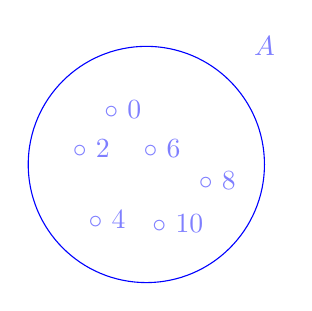
\begin{tikzpicture}
			      \begin{scope}[shift={(3cm,-5cm)}, fill opacity=0.5]
				      \draw[blue] (0,0) circle (1.5cm);
				      \draw[blue] (1.5,1.5) node {$A$};
				      \draw[blue] (-0.3,0.7) node {$\circ\ 0$};
				      \draw[blue] (-0.7,0.2) node {$\circ\ 2$};
				      \draw[blue] (-0.5,-0.7) node {$\circ\ 4$};
				      \draw[blue] (0.4,-0.75) node {$\circ\ 10$};
				      \draw[blue] (0.9,-0.2) node {$\circ\ 8$};
				      \draw[blue] (0.2,0.2) node {$\circ\ 6$};
			      \end{scope}
		      \end{tikzpicture}
	      \end{displaymath}
\end{enumerate}
\Def{Sia $\A$ un insieme finito.}{La \ul{\textbf{cardinalità}} di $\A$ è i numero di elementi di $\A$ e si denota $|\A|$\\
	\begin{itemize}
		\item Insieme vuoto: insieme che non contiene nessun elemento, si denota con $\emptyset$, $\{\}$ e ha cardinalità $|\emptyset|=0$
	\end{itemize}}
\subsubsection*{\color{blue}\ul{I principali insiemi numerici}}
$\mathbb{N}=\{0,1,2,3,\cdots\}$: numeri naturali\\
$\mathbb{Z}=\{\cdots,-3,-2,-1,0,1,2,3,\cdots\}$: numeri naturali\\
$\mathbb{Q}=\{\frac{a}{b}:a,b$ e $\mathbb{Z},b\not=0\}$: numeri razionali\\
$\R$: numeri reali\\
$\mathbb{C}$: numeri complessi
\subsubsection*{\color{blue}\ul{Inclusione di insiemi}}
\begin{itemize}
	\item $\A\subseteq\B\quad(\A$ è contenuto in $\B)\Leftrightarrow(\forall x,x\in\A\Rightarrow x\in\B)$\\
	      {\color{violet}$\B\supseteq\A("\B$ contiene $\A")$}\\
	      Se $\A\subseteq\B$, diciamo che $\A$ è un \ul{sottoinsieme} di $\B$
	      \Esempio{$\mathbb{N}\subseteq\mathbb{Z}\subseteq\mathbb{Q}\subseteq\R\subseteq\mathbb{C}$}
	\item $\A=\B\Leftrightarrow(x\in\A\Leftrightarrow x\in\B)\Leftrightarrow(\underbrace{\A\subseteq\B\wedge\B\subseteq\A}_{\colort{violet}{doppia inclusione}})$
\end{itemize}
\subsubsection*{\color{blue}\ul{Operazioni tra insiemi}}
Siano $\A$ e $\B$ due insiemi
\begin{enumerate}
	\item \ul{Intersezione} \color{violet}$\leftrightarrow\wedge$\color{default}:\\
	      $\A\cap\B:=\{x:x\in\A\underset{\text{"e"}}{\wedge} x\in\B\}$\\
	      Se $\A\cap\B=\emptyset$ allora $\A$ e $\B$ sono detti \ul{disgiunti}\\
	      \ul{Proprietà}:
	      \begin{itemize}
		      \item $\A\cap\emptyset=\emptyset$
		      \item $\A\cap\B=\B\cap\A$
		      \item $\A\subseteq\B\Rightarrow\A\cap\B=\A$
	      \end{itemize}
	\item \ul{Unione} \color{violet}$\leftrightarrow\vee$\color{default}:\\
	      $\A\cup\B:=\{x:x\in\A\vee x\in\B\}$\\
	      \ul{Proprietà}:
	      \begin{itemize}
		      \item $\A\cup\emptyset=\A$
		      \item $\A\cup\B=\B\cup\A$
		      \item $\A\subseteq\B\Rightarrow\A\cup\B=\B$
		      \item $\A\subseteq\A\cup\B,\B\subseteq\A\cup\B$
	      \end{itemize}
	\item \ul{Differenza} \color{violet}$\leftrightarrow\backslash$\color{default}:\\
	      $\B\backslash\A:=\{x:x\in\B\wedge x\not\in\A\}$\\
	      \ul{Proprietà}:
	      \begin{itemize}
		      \item $\A\backslash\emptyset=\A$
		      \item $\emptyset\backslash\A=\A$
	      \end{itemize}
	\item \ul{Prodotto cartesiano} \color{violet}$\leftrightarrow\times$\color{default}:\\
	      $\A\times\B:=\{\underbrace{(a,b)}_{\text{coppie ordinate}}:a\in\A,b\in\B\}$\\
	      \ul{Proprietà}:
	      \begin{itemize}
		      \item $|\A\times\B|=|\A|\cdot|\B|$
		      \item $\A\times\emptyset=\emptyset=\emptyset\times\A$
	      \end{itemize}
	      $\A_1,\cdots,\A_n$ insiemi\\
	      $\A_1\times\cdots\times\A_n=\{(a_1,\cdots,a_n):a_i\in\A_i,\forall i\}$
\end{enumerate}
\subsection{\texorpdfstring{\color{blue}\ul{Funzioni}}{Funzioni}}
\Def{Siano $\A,\B$ due insiemi:}
{Una funzione $f:\A\rightarrow\B$ è una legge che associa \ul{ad ogni} elemento di $\A$, \ul{uno ed un solo} elemento di $\B$.\\
	$f:\overset{\text{dominio}}{\A}\underset{x\mapsto y}{\rightarrow}\overset{\text{codominio}}{\B}$\\
	Se $y=f(x),\ x\in\A$, allora $y$ è \ul{l'immagine} di $x$ e $x$ è la \ul{controimmagine} di $y$
	\Esempio{
		$\A=\{1,2,3\}\\\B=\{a,b,c,d\}$\\\\
		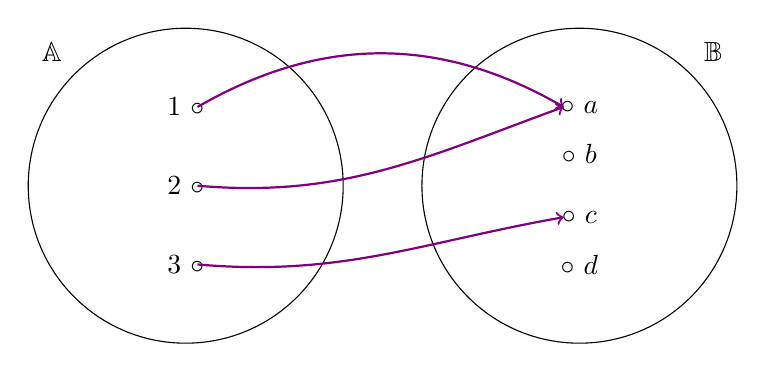
\begin{tikzpicture}
			\draw (0,0) circle (2);
			\draw (-1.7,1.7) node {$\A$};
			\draw (0,1) node {$1\ \circ$};
			\draw (0,0) node {$2\ \circ$};
			\draw (0,-1) node {$3\ \circ$};
			\draw (5,0) circle (2);
			\draw (6.7,1.7) node {$\B$};
			\draw (5,1) node   {$\circ\ a$};
			\draw (5,0.4) node {$\circ\ b$};
			\draw (5,-0.4) node{$\circ\ c$};
			\draw (5,-1) node  {$\circ\ d$};

			\draw[violet,thick,->] (0.15,1) to[out=30,in=150] (4.80,1);
			\draw[violet,thick,->] (0.15,0) to[out=-5,in=200] (4.80,1);
			\draw[violet,thick,->] (0.15,-1) to[out=-5,in=190] (4.80,-0.4);
		\end{tikzpicture}\\\\
		$f:\A\longrightarrow\B$\\
		\hspace*{1.5em}\begin{minipage}{.8\textwidth}$1\longmapsto a\\2\longmapsto a\\3\longmapsto c$\end{minipage}
	}\\\\
	$a$ è \ul{l'}immagine di $1$ e $2\qquad(f(1)=a=f(2))$\\
	$1$ è \ul{una} controimmagine di $a$
}
\Def{Sia $f:\A\rightarrow\B$ una funzione e sia $\mathbb{X}\subseteq\A$:}
{$f(x):=\{f(x):x\in\mathbb{X}\}$ è l'immagine di $\mathbb{X}$ tramite $f$\\
	$Im(f):=f(\A)$ è l'immagine della funzione}
\label{sec:lezione-2}
\section{09/03/22}
\subsection{\texorpdfstring{\color{blue}\ul{Funzioni (continuo)}}{Funzioni (continuo)}}
\Def{Una funzione $f:\A\rightarrow\B$ si dice \ul{iniettiva} se $\forall x,y\in\A$}{$$\underset{\text{\color{cyan}(elementi distinti di $\A$ hanno immagini distinte)}}{x\ne y\Rightarrow f(x)\ne f(y)}$$$$\Updownarrow$$$$\hspace*{8em}f(x)=f(y)\Rightarrow x=y:\color{purple}\begin{cases}\text{usiamo questa} \\\text{implicazione}\\\text{per dimostrare}\\\text{che una funzione}\\\text{è iniettiva}
		\end{cases}$$\colort{orange}{(ogni elemento di $\B$ ha \ul{al più} una controimmagine)}}
\Def{Una funzione $f:\A\rightarrow\B$ si dice \ul{suriettiva} se $Im(f)=\B$,}{o equivalentemente se $\forall y\in\B,\exists x\in\A:f(x)=y$\\\colort{orange}{(ogni elemento di $\B$ ha \ul{almeno} una controimmagine)}}
\Def{Una funzione $f:\A\rightarrow\B$ si dice \ul{biettiva} o \ul{biunivoca}}{se è al tempo stesso iniettiva \ul{e} suriettiva\\\colort{orange}{(ogni elemento di $\B$ ha \ul{esattamente} una controimmagine)}}
\Esempio{$f:\R\rightarrow\R\\\hspace*{1.5em}x\rightarrow x^2$
	\begin{itemize}
		\item \colort{cyan}{È iniettiva? No, perchè $f(-1)=1=f(1)$}
		\item \colort{violet}{È suriettiva? No, perchè $f(x)=x^2\geq0\forall x\in\R\Rightarrow Im(f)\subseteq\R^+\Rightarrow Im(f)\not=\R$}
	\end{itemize}}
\vspace*{1em}
\subsubsection{\texorpdfstring{\color{blue}\ul{Nozione di campo}}{\ul{Nozione di campo}}}
\Def{Se un insieme possiede delle operazioni che verificano certe proprietà, è una struttura algebrica.}{}
\Def{Sia $\X$ un insieme.}{Un'\ul{operazione binaria interna} è una funzione dal prodotto cartesiano $\X\times \X$ in $\X$.\\\\$*:\X\times\X\rightarrow\X$\\\hspace*{1.4em}$(x,y)\rightarrow x*y$}\\\vspace{1em}\\
L'addizione su $\R$ è un'operazione binaria interna\\$+:\R\times\R\rightarrow\R$\\\hspace*{-0.7em}$\qquad(x,y)\rightarrow x+y$\\\\
	\colort{purple}{\ul{Proprietà di $(\R,+)$}}
	\begin{enumerate}
		\item Commutatività: $x+y=y+x,\forall x,y\in\R$
		\item Associatività: $(x+y)+z=x+(y+z),\forall x,y,z\in\R$
		\item Elemento neutro: $\exists0\in\R:\ x+0=0+x=x,\ \forall x\in\R$
		\item Opposto: $\forall x\in\R,\ \exists x'\in\R:\ x+x'=x'+x=0\ \color{violet}(x'=-x)$
	\end{enumerate}
	Anche la moltiplicazione su $\R$ è un'operazione binaria interna\\
$\cdot:\R\times\R\rightarrow\R$\\
	\hspace*{1.5em}$(x,y)\rightarrow x\cdot y$\\\\
	\colort{purple}{\ul{Proprietà di $(\R,\cdot)$}}
	\begin{enumerate}
		\item Commutatività: $x\cdot y=y\cdot x,\forall x,y\in\R$
		\item Associatività: $(x\cdot y)\cdot z=x\cdot(y\cdot z),\forall x,y,z\in\R$
		\item Elemento neutro: $\exists1\in\R:\ x\cdot1=1\cdot x,\ \forall x\in\R$
		\item Elemento inverso: $\forall x\in\R\backslash\{0\},\ \exists x'\in\R:\ x\cdot x'=x'\cdot x=1$ \colort{violet}{$(x'=x^{-1}=\frac{1}{x})$}
	\end{enumerate}
	Infine $+$ e $\cdot$ soddisfano la proprietà distributiva:\\
$\forall x,y,z\in\R,x\cdot(y+z)=x\cdot y+x\cdot z$\\\\
	\colort{green}{$\R$ dotato delle operazioni di addizione e moltiplicazione è chiamato \ul{campo} dei numeri reali.}\\
	\colort{purple}{Più in generale abbiamo (definizione di campo)}
	\Def{Sia $\K\ne\emptyset$ un insieme dotato di due operazioni binarie:}{
		\begin{itemize}
			\item $+:\K\times\K\rightarrow\K$
			\item $\cdot:\K\times\K\rightarrow\K$
		\end{itemize}}\\\\
$(\K,+,\cdot)$ è detto un \ul{campo} se\\
	\begin{enumerate}
		\item $+$ è commutativa \qquad\colort{violet}{$(\forall x,y\in\K,\ x+y=y+x)$}
		\item $+$ è associativa \qquad\colort{violet}{$(\forall x,y,z\in\K,\ (x+y)+z=x+(y+z))$}
		\item esiste elemento neutro $0$ rispetto a $+$ \qquad\colort{violet}{$(0+x=x+0=x,\forall x\in\K)$}
		\item $\forall x\in\K$ esiste un opposto \qquad\colort{violet}{$(x':\ x+x'=x'+x=0)$}
		\item $\cdot$ è commutativa \qquad\colort{violet}{$(\forall x,y\in\K,\ x\cdot y=y\cdot x)$}
		\item $\cdot$ è associativa \qquad\colort{violet}{$(\forall x,y,z\in\K,\ (x\cdot y)\cdot z=x\cdot (y\cdot z))$}
		\item esiste elemento neutro $1$ rispetto a $\cdot$ \qquad\colort{violet}{$(x\cdot1=1\cdot x=x,\ \forall x\in\K)$}
		\item $\forall x\in\K\backslash\{0\}$ esiste un inverso \qquad\colort{violet}{$(x':\ x\cdot x'=x'\cdot x=1)$}
		\item $\cdot$ è distributiva rispetto a $+$ \qquad\colort{violet}{$(\forall x,y,z\in\K,\ x\cdot(y+z)=x\cdot y+x\cdot z)$}
	\end{enumerate}

	\Esempio{$\mathbb{F}_2=\{0, 1\}$\colort{purple}{: campo finito a due elementi}
		\begin{itemize}
			\item $\cdot:\mathbb{F}_2\cdot\mathbb{F}_2\rightarrow\mathbb{F}_2$\\
			      \hspace*{1.8em}$(0,0)\rightarrow 0$\\
			      \hspace*{1.8em}$(0,1)\rightarrow 0$\\
			      \hspace*{1.8em}$(1,0)\rightarrow 0$\\
			      \hspace*{1.8em}$(1,1)\rightarrow 1$
			\item $+:\mathbb{F}_2\times\mathbb{F}_2\rightarrow\mathbb{F}_2$\\
			      \hspace*{1.8em}$(0,0)\rightarrow 0$\\
			      \hspace*{1.8em}$(0,1)\rightarrow 1$\\
			      \hspace*{1.8em}$(1,0)\rightarrow 1$\\
			      \hspace*{1.8em}$(1,1)\rightarrow 1$
		\end{itemize}
		$0$ è l'elemento neutro di $+$\\
		$1$ è l'elemento neutro di $\cdot$\\
		$1$ è l'opposto e l'inverso di se stesso.\\
		È possibile verificare che $+$ e $\cdot$ verificano $1,2,\cdots,9$.
	}
	\subsection{Algebra lineare}
	Wikipedia:
	\begin{quotation}
		Branca della matematica che si occupa dello studio di spazi vettoriali (o anche detti spazi lineari), di trasformazioni lineari e di sistemi di equazioni lineari.
	\end{quotation}
	Molti problemi di matematica e fisica verificano la seguente proprietà:\\
	Se $v,w\in\mathbb{X}$ sono due soluzioni del problema, allora anche $v+w$ e $\lambda v,\lambda\in\R$  ($+$ e $\cdot$ operazioni su $\mathbb{X}$) sono soluzioni del problema.\\
	Problemi di questo tipo sono detti \textit{lineari}.

	\subsubsection*{\colort{blue}{Nozione base dell'algebra lineare: \ul{spazio vettoriale}}}

	I \colort{violet}{vettori} sono usati in fisica per rappresentare grandezze fisiche caratterizzate da:
	\begin{itemize}
		\item una direzione
		\item un verso
		\item un'intensità
	\end{itemize}
	Tali grandezze sono dette \ul{vettoriali}:
	\ul{esempi}: velocità, forza, accelerazione, campo elettrico, momento angolare.

$\begin{bmatrix}
	\text{si differenziano dalle \textbf{grandezze scalari} che sono definite unicamente dall'intensità} \\
	\text{\ul{esempi}: massa, temperatura, volume, lavoro, pressione, etc...}                            \\
\end{bmatrix}$\vspace{1em}\\
	GEOMETRICAMENTE rappresentiamo un vettore con un \textbf{segmento orientato}\\
	\colort{green}{Nel piano euclideo $\Pi$:}\\

	
\begin{tikzpicture}
		\begin{scope}
			\draw[->] (-1,0) -- (2,1.5);
			\draw (-1.2,0.025) node {$A$};
			\draw (2.2,1.55) node {$B$};
			\draw[purple] (-4, 1) node {punto di};
			\draw[purple] (-4, 0.5) node {applicazione o};
			\draw[purple] (-4, 0) node {iniziale};
			\path[purple,->] (-2.8,0.6) edge[bend left] node [right] {} (-1.4,0.2);
			\draw[purple] (4.5, 1.7) node {punto finale};
			\path[purple,->] (3.5,1.7) edge[bend right] node [left] {} (2.5,1.65);
		\end{scope}
	\end{tikzpicture}
	\Def{Un \ul{segmento orientato} è una coppia ordinata di punti $(A,B)\in\Pi\times\Pi$.}{Notazione: $\overrightarrow{AB}:=(A,B)$}\vspace{1em}\\
$\begin{array}{ccc}
	\colort{cyan}{\ul{FISICA}} &                 & \colort{violet}{\ul{GEOMETRIA}}                                        \\
	\colort{cyan}{direzione}   & \leftrightarrow & \colort{violet}{qualsiasi retta parallela al segmento $\overline{AB}$} \\
	\colort{cyan}{verso}       & \leftrightarrow & \colort{violet}{punto iniziale $\rightarrow$ finale}                   \\
	\colort{cyan}{intensità}   & \leftrightarrow & \colort{violet}{lunghezza di $\overline{AB}$}                          \\
\end{array}$\vspace{1em}\\
	\ul{Nota}: $\forall P\in\pi,\ \overrightarrow{PP}$ corrisponde al vettore nullo (per cui non è possibile definire né una direzione né un verso)\\
	Nel piano esistono infiniti segmenti orientati che hanno \textit{stessa direzione, stesso verso, stessa intensità}.\\
	Diciamo che questi segmenti orientati sono \textit{equipollenti} due a due.\vspace{1em}\\
	Più formalmente:\Def{Due segmenti orientati $\overrightarrow{AB}$ e $\overrightarrow{CD}$ si dicono \ul{equipollenti}}{e scriviamo $\overrightarrow{AB}\thicksim\overrightarrow{CD}$ se il quadrilatero avente vertici, ordinatamente $ABCD$ è un parallelogramma.}

	L'equipollenza è una \ul{relazione di equivalenza}:
	\begin{itemize}
		\item riflessiva \colort{violet}{(ogni segmento orientato è equipollente a se stesso: $\overrightarrow{AB}\thicksim\overrightarrow{AB}$)}
		\item simmetrica \colort{violet}{(se $\overrightarrow{AB}\thicksim\overrightarrow{CD}$ allora $\overrightarrow{CD}\thicksim\overrightarrow{AB}$)}
		\item transitiva \colort{violet}{(se $\overrightarrow{AB}\thicksim\overrightarrow{CD}$ allora $\overrightarrow{CD}\thicksim\overrightarrow{EF}$ allora $\overrightarrow{AB}\thicksim\overrightarrow{EF}$)}
	\end{itemize}

	Per ogni segmento orientato $\overrightarrow{AB}$ posso considerare la corrispondente classe di equipollenza: $$\text{Classe }\overrightarrow{AB}=\underset{\underset{\underset{\colort{violet}{equivalenti ad $\overrightarrow{AB}$.}}{\colort{violet}{insieme dei segmenti orientati}}}{\uparrow}}{\{\overrightarrow{CD}:\ \overrightarrow{AB}\thicksim\overrightarrow{CD}\}}$$

	\begin{displaymath}
		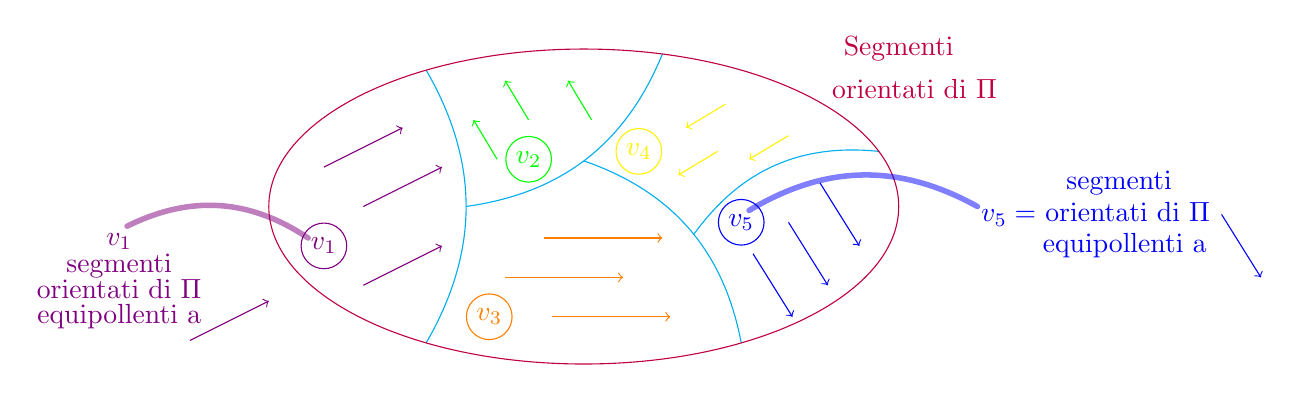
\begin{tikzpicture}
			\begin{scope}[cyan] % barriers
				\path (-2,-1.73) edge[bend right] node [left] {} (-2,1.73);
				\path (-1.5,0) edge[bend right] node [left] {} (1,1.94);
				\path (0,0.58) edge[bend left] node [right] {} (2,-1.73);
				\path (1.4,-0.35) edge[bend left] node [right] {} (3.75,0.7);
			\end{scope}
			% vectors
			\begin{scope}[shift={(-3.3,-0.5)}, violet]
				\draw (0,0) node {\tikz[baseline=(char.base)]{\node[shape=circle,draw,inner sep=2pt] (char) {$v_1$};}};
				\draw[->] (0.5,-0.5) -- (1.5,0);
				\draw[->] (0.5,0.5) -- (1.5,1);
				\draw[->] (0,1) -- (1,1.5);
			\end{scope}
			\begin{scope}[shift={(-0.7,0.6)}, green]
				\draw (0,0) node {\tikz[baseline=(char.base)]{\node[shape=circle,draw,inner sep=2pt] (char) {$v_2$};}};
				\draw[->] (-0.4,0) -- (-0.7,0.5);
				\draw[->] (0,0.5) -- (-0.3,1);
				\draw[->] (0.8,0.5) -- (0.5,1);
			\end{scope}
			\begin{scope}[shift={(-1.2,-1.4)}, orange]
				\draw (0,0) node {\tikz[baseline=(char.base)]{\node[shape=circle,draw,inner sep=2pt] (char) {$v_3$};}};
				\draw[->] (0.8,0) -- (2.3,0);
				\draw[->] (0.2,0.5) -- (1.7,0.5);
				\draw[->] (0.7,1) -- (2.2,1);
			\end{scope}
			\begin{scope}[shift={(0.7,0.7)}, yellow]
				\draw (0,0) node {\tikz[baseline=(char.base)]{\node[shape=circle,draw,inner sep=2pt] (char) {$v_4$};}};
				\draw[->] (1.9,0.2) -- (1.4,-0.1);
				\draw[->] (1,0) -- (0.5,-0.3);
				\draw[->] (1.1,0.6) -- (0.6,0.3);
			\end{scope}
			\begin{scope}[shift={(2,-0.2)}, blue]
				\draw (0,0) node {\tikz[baseline=(char.base)]{\node[shape=circle,draw,inner sep=2pt] (char) {$v_5$};}};
				\draw[->] (1,0.5) -- (1.5,-0.3);
				\draw[->] (0.6,0) -- (1.1,-0.8);
				\draw[->] (0.15,-0.4) -- (0.65,-1.2);
			\end{scope}
			\draw[purple] (0,0) ellipse (4 and 2);
			\draw[purple] (4,2) node {Segmenti};
			\draw[purple] (4.2,1.5) node {orientati di $\Pi$};
			\begin{scope}[shift={(2.1,-0.05)}, blue] %v5 explaination
				\path[line width=2, opacity=0.5, line cap=round] (0,0) edge[bend left] node [right] {} (2.9,0.05);
				\draw (4.4,-0.05) node {$v_5=$ orientati di $\Pi$};
				\draw (4.7,0.35) node {segmenti};
				\draw (4.77,-0.45) node {equipollenti a};
				\draw[->] (6,-0.05) -- (6.5,-0.85);
			\end{scope}
			\begin{scope}[shift={(-3.5,-0.4)}, violet] %v1 explaination
				\path[line width=2, opacity=0.5, line cap=round] (0,0) edge[bend right] node [left] {} (-2.3,0.15);
				\draw (-2.4,-0.05) node {$v_1$};
				\draw (-2.4,-0.35) node {segmenti};
				\draw (-2.4,-0.65) node {orientati di $\Pi$};
				\draw (-2.4,-1) node {equipollenti a};
				\draw[->] (-1.5,-1.3) -- (-0.5,-0.8);
			\end{scope}
		\end{tikzpicture}
	\end{displaymath}

	\Def{Un \ul{vettore geometrico} del piano $\Pi$ è una classe di equipollenza}{}\\
	Sia $O\in\Pi$ un punto fissato. Mostriamo che per ogni vettore geometrico (= classe di equipollenza) possiamo trovare un "rappresentante" con punto di applicazione O.\\
	Basta mostrare che per ogni segmento orientato $\overrightarrow{AB}$ esiste un punto $P\in\Pi$ tale che $\overrightarrow{OP}$ è equivalente ad $\overrightarrow{AB}$.
	\begin{displaymath}
		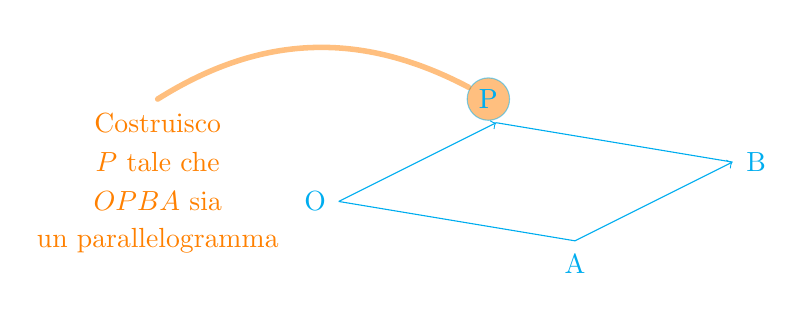
\begin{tikzpicture}
			\begin{scope}[cyan]
				\draw[->] (0,0) -- (2,1);
				\draw (-0.3,0) node {O};
				\draw (1.9,1.3) node[shape=circle,draw,fill=orange,opacity=0.5,inner sep=2pt] {P};
				\draw (1.9,1.3) node {P};
				\path[orange,line width=2, opacity=0.5, line cap=round] (1.65,1.45) edge[bend right] node [left] {} (-2.3,1.3);
				\begin{scope}[shift={(-2.3,0)},orange]
					\draw (0,1) node {Costruisco};
					\draw (0,0.5) node {$P$ tale che};
					\draw (0,0) node {$OPBA$ sia};
					\draw (0,-0.5) node {un parallelogramma};
				\end{scope}
				\draw[->] (3,-0.5) -- (5,0.5);
				\draw (3,-0.8) node {A};
				\draw (5.3,0.5) node {B};
				\draw (3,-0.5) -- (0,0);
				\draw (2,1) -- (5,0.5);
			\end{scope}
		\end{tikzpicture}
	\end{displaymath}
	Per transitività, $\overrightarrow{OP}$ è equipollente a tutti i segmenti orientati equipollenti a $\overrightarrow{AB}$ e posso sceglierlo come \ul{rappresentante} della classe di equipollenza di $\overrightarrow{AB}$.\\
	Sia $\V=\{\text{vettori geometrici del piano}\}$\\
	Abbiamo quindi una funzione biunivoca:\\
	$$\V=\begin{Bmatrix}\text{vettori geometrici}\\\text{del piano}\end{Bmatrix}\leftrightarrow\begin{Bmatrix}\text{segmenti orientati}\\\overrightarrow{OP},\ P\in\Pi\end{Bmatrix}$$
	$$\begin{matrix}\underset{\colort{gray}{(classe di equipollenza)}}{v}&\longmapsto&\begin{matrix}\text{rappresentante di}\\\text{$v$ con punto di}\\\text{applicazione $O$}\end{matrix}\\\begin{matrix}\text{classe}\\\text{di equipollenza}\\\text{di }\overrightarrow{OP}\end{matrix}&\longleftarrow\!\shortmid&\overrightarrow{OP}\end{matrix}$$
	A partire da ora lavoreremo solo con segmenti orientati aventi lo stesso punto di applicazione.
	\section{15/03/22}
	Nella \colort{blue}{\ul{\hyperref[sec:lezione-2]{Lezione 2}}} abbiamo definito un \ul{vettore geometrico} (nel piano) come una classe di equipollenza di segmenti orientati (del piano) e, fissato un punto $O\in\Pi$ , abbiamo costruito una biezione:
	$$\V=\begin{Bmatrix}\text{vettori geometrici}\\\text{del piano}\end{Bmatrix}\longleftrightarrow\begin{Bmatrix}\text{segmenti orientati}\\\overrightarrow{OP},\ P\in\Pi\end{Bmatrix}$$
	Questa biezione ci permette in particolare, di rappresentare ogni vettore con un segmento orientato $\overrightarrow{OP}$, con un \uwave{abuso di notazione}, scriveremo
	$$\V=\{\text{segmenti orientati }\overrightarrow{OP},P\in\pi\}$$
	e chiameremo \ul{vettori} gli elementi di $\V$.\\Notiamo che $\forall\overrightarrow{v}\in\V,\exists P\in\Pi:\overrightarrow{v}=\overrightarrow{OP}$\\
	\subsection{\colort{violet}{Operazioni su $\V$}}
	\begin{itemize}
		\item \colort{cyan}{\ul{Somma di vettori}}\\
		      Siano $\overrightarrow{v},\overrightarrow{w}\in\V$ e siano $P,Q\in\Pi:$\\
		      \colort{purple}{$\overrightarrow{v}=\overrightarrow{OP}$} e \colort{purple}{$\overrightarrow{w}=\overrightarrow{OQ}$\vspace*{1em}}\\
		      Definiamo\\
		      \colort{violet}{$\overrightarrow{v}+\overrightarrow{w}=\overrightarrow{OR}$}, tale che $OPRQ$ sia un parallelogramma. \colort{green}{(regola del parallelogramma)}\\
		      \begin{displaymath}
			      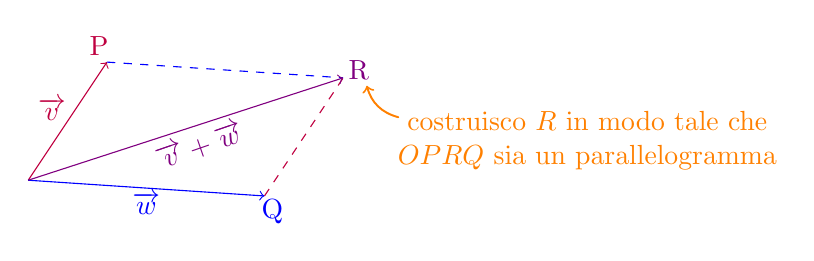
\begin{tikzpicture}
				      \begin{scope}[purple]
					      \draw[->] (0,0) -- (1,1.5);
					      \draw (0.3,0.9) node {$\overrightarrow{v}$};
					      \draw (0.9,1.7) node {P};
					      \draw[dashed] (3,-0.2) -- (4,1.3);
				      \end{scope}
				      \begin{scope}[blue]
					      \draw[->] (0,0) -- (3,-0.2);
					      \draw (1.5,-0.3) node {$\overrightarrow{w}$};
					      \draw (3.1,-0.4) node {Q};
					      \draw[dashed] (1,1.5) -- (4,1.3);
				      \end{scope}
				      \begin{scope}[violet]
					      \draw[->] (0,0) -- (4,1.3);
					      \begin{turn}{19}
						      \draw (2.2,-0.3) node {$\overrightarrow{v}+\overrightarrow{w}$};
					      \end{turn}
					      \draw (4.2,1.4) node {R};
					      \begin{scope}[orange]
						      \path[line width=0.7, line cap=round,->] (4.7,0.8) edge[bend left] node [right] {} (4.3,1.2);
						      \draw (7.1,0.5) node {$\begin{matrix}\text{costruisco $R$ in modo tale che}\\OPRQ\text{ sia un parallelogramma}\end{matrix}$};
					      \end{scope}
				      \end{scope}
			      \end{tikzpicture}
		      \end{displaymath}
		      \ul{Nota}: E se $O,\ P$ e $Q$ fossero collineari (giacciono sulla stessa retta)?\\
		      \hspace*{2.5em}
		      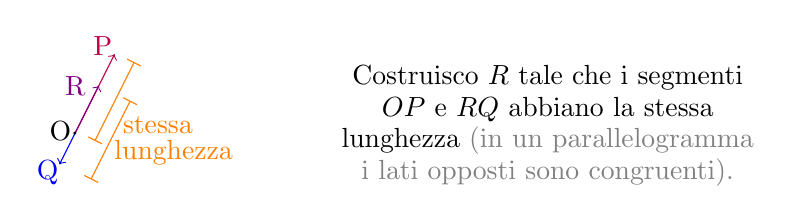
\begin{tikzpicture}
			      \begin{scope}
				      \draw[purple,->] (0,0) -- (0.5,1);
				      \draw[purple] (0.35,1.1) node {P};
				      \draw[blue,->] (0,0) -- (-0.2,-0.4);
				      \draw[blue] (-0.35,-0.5) node {Q};
				      \draw[violet,->] (0,0) -- (0.3,0.6);
				      \draw[violet] (0,0.6) node {R};
				      \draw (-0.14,0.027) node {O$\cdot$};
				      \begin{scope}[orange,shift={(0.25,-0.1)}]
					      \draw[|-|] (0,0) -- (0.5,1);
					      \draw[|-|,shift={(0.15,-0.09)}] (-0.2,-0.4) -- (0.3,0.6);
					      \draw (0.8,0.2) node {stessa};
					      \draw (1,-0.15) node {lunghezza};
				      \end{scope}
			      \end{scope}
						\begin{scope}[shift={(6,0.7)}]
							\draw (0,0) node {Costruisco $R$ tale che i segmenti};
							\draw (0,-0.4) node {$OP$ e $RQ$ abbiano la stessa};
							\draw (0,-0.8) node {lunghezza \colort{gray}{(in un parallelogramma}};
						\draw[gray] (0,-1.2) node {i lati opposti sono congruenti).};
						\end{scope}
		      \end{tikzpicture}\\
		      Otteniamo così un'\ul{operazione binaria interna}:\\
		      \colort{purple}{$+:\V\times\V\longrightarrow\V$}\\
		      \hspace*{1em}\colort{purple}{$(\overrightarrow{v},\overrightarrow{w})\mapsto\overrightarrow{v}+\overrightarrow{w}$}
				\item \colort{cyan}{\ul{Moltiplicazione per scalari}}\\
		      Sia $\overrightarrow{v}\in\V$ e sia $P\in\Pi:\overrightarrow{v}=\overrightarrow{OP}$. Sia $\lambda\in\R$.\vspace*{1em}\\
		      Definiamo $\lambda\cdot\overrightarrow{v}=\overrightarrow{OR}$\\tale che
		      \begin{itemize}
			      \item $O,P,R$ sono collineari (sulla stessa retta)
			      \item $\overline{OR}=|\lambda|\overline{OP}$
			      \item $\overrightarrow{OR}$ è orientato concordemente a $\overrightarrow{OP}\\\overrightarrow{OR}$ è orientato discordemente a $\overrightarrow{OP}$ se\\
			            $\lambda<0\vee\lambda=0,R=O$\\
			            Questa è un'operazione binaria \ul{esterna}:\\
			            $\cdot:\R\times\V\rightarrow \V$\\
			            \hspace*{1.5em}$(\lambda,\overrightarrow{v})\rightarrow\lambda\cdot\overrightarrow{v}$
		      \end{itemize}
	\end{itemize}
	\subsection{Piano Cartesiano}
	\par$\{P:P\in\pi\}\leftrightarrow\{(x,y):x,y\in\R\}=\R^2$\\
$\V=\{$segmenti orientati $\overrightarrow{OP},P\in\pi\}=\{$vettori geometrici nel piano$\}$\\
	In particolare esiste una biezione:\\
$\V\leftrightarrow\R^2$\\
$\forall P\in\pi,\overrightarrow{OP}\rightarrow(x,y)$, dove $x,y$ sono rispettivamente ascissa e ordinata di $P$\\
$\overrightarrow{OP}\leftarrow(x,y)$ dove $P(x,y)$\\
	Vogliamo tradurre le operazioni su $\V$ in operazioni su $\R^2$:
	\begin{enumerate}
		\item $\overrightarrow{v}=\overrightarrow{OP},P(x_P,y_P)$\\
		      $\overrightarrow{w}=\overrightarrow{OQ},Q(x_Q,y_Q)$
		      $\overrightarrow{v}+\overrightarrow{w}=\overrightarrow{OR}:$ quali sono le coordinate di $R$?\\
		      $OPQR\Rightarrow A(x_A,y_A)$ parallelogramma con punto medio di $PQ$ e $OR$\\
		      $A$ punto medio di $PQ\Rightarrow\{x_A=\frac{x_P+x_Q}{2},y_A=\frac{y_P+x_Q}{2}\}$\\
		      $A$ punto medio di $OR\Rightarrow\{x_A=\frac{x_R}{2},y_A=\frac{y_R}{2}\}$\\
		      $\Rightarrow\{x_R=x_P+x_Q,y_R=y_P+y_Q\}$\\
		      Operazione binaria \ul{interna}:\\
		      $+:\R^2\times\R^2\rightarrow\R^2$\\
		      $((x_1,y_1),(x_2,y_2))\mapsto(x_1+x_2,y_1+y_2)$
		\item $\overrightarrow{v}\in\V,\overrightarrow{v}=\overrightarrow{OP},P(x_P,y_P),\lambda\in\R$\\
		      $\lambda\cdot\overrightarrow{v}=\overrightarrow{OR}:$ quali sono le coordinate di $R$?\\
		      $\overrightarrow{OR}=\lambda\cdot\overrightarrow{OP}$\\
		      $OPH$ e $ORK$ sono simili per costruzione con rapporto di proporzioni $|\lambda|$.\\
		      \ul{Due casi}:
		      \begin{enumerate}
			      \item $\lambda\ge0$ $\overrightarrow{OR}$ è concord con $\overrightarrow{OP}$ e quindi:\\
			            $x_R=|\lambda|x_P=\lambda x_P$\\
			            $y_R=|\lambda|y_P=\lambda y_P$
			      \item $\lambda<0$ $\overrightarrow{OR}$ è discorde con $\overrightarrow{OP}$ e quindi:\\
			            $x_R=-|\lambda|x_P=\lambda x_P$\\
			            $y_R=-|\lambda|y_P=\lambda y_P$
		      \end{enumerate}
		      Operazione binaria \ul{esterna}:\\
		      $\cdot:\R\times\R^2\rightarrow\R^2$\\
		      \hspace*{0.1em}$(y,(x,y))\mapsto\lambda\cdot(x,y):=(\lambda x,\lambda y)$
	\end{enumerate}
	In conclusione abbiamo definito due operazioni su $\R^2$ "compatibili" con le operazioni definite su $\V$:
	\begin{itemize}
		\item $+: \R^2\times\R^2\rightarrow\R^2$\\$((x_1,y_1),(x_2,y_2))\mapsto(x_1,y_1)+(x_2,y_2):=(x_1+y_1,x_2+y_2)$
		\item $\cdot: \R^2\times\R^2\rightarrow\R^2$\\\hspace*{-0.3em}$(\lambda,(x_2,y_2))\mapsto\lambda\cdot(x_2,y_2):=(\lambda\cdot x,\lambda\cdot y)$
	\end{itemize}
	\ul{Proprietà} di $+$ e $\cdot$ :
	\begin{enumerate}
		\item Commutatività:\\$\forall(x_1,y_1),(x_2,y_2)\in\R^2, (x_1,y_1)+(x_2,y_2)=(x_2,y_2)+(x_1,y_1)$
		\item Associatività:\\$\forall(x_1,y_1),(x_2,y_2),(x_3,y_3)\in\R^2,\\((x_1,y_1)+(x_2,y_2))+(x_3,y_3)=(x_1,y_1)+((x_2,y_2)+(x_3,y_3))$
		\item Elemento neutro $(+)$:\\$(0,0)\in\R^2$ è tale che $(x,y)+(0,0)=(0,0)+(x,y)=(x,y)$
		\item Elemento opposto:\\$\forall(x,y)\in\R^2,\exists(x',y')\in\R^2:(x,y)+(x',y')=(x',y')+(x,y)=(0,0)$
		\item Distributività rispetto a vettori:\\$\forall(x_1,y_1),(x_2,y_2)\in\R^2,\forall\lambda\in\R$\\$\lambda\cdot((x_1,y_1)+(x_2,y_2))=\lambda\cdot(x_1,y_1)+\lambda\cdot(x_2,y_2)$
		\item Distributività rispetto a scalari:\\$\forall(x,y)\in\R^2,\forall\lambda,\mu\in\R$\\$(\lambda+\mu)\cdot(x,y)=\lambda\cdot(x,y)+\mu\cdot(x,y)$
		\item Senza nome:\\$\lambda\mu\cdot(x,y)=\lambda\cdot(\mu\cdot(x,y))$
		\item Elemento neutro $(\cdot)$:\\$1\cdot(x,y)=(x,y)\forall(x,y)\in\R^2$
	\end{enumerate}
$(\R^2,+,\cdot)$ è il primo esempio di "spazio vettoriale" su $\R$.\vspace*{1em}\\
	Più in generale uno spazio vettoriale (o spazio lineare) è una struttura algebrica composta da:
	\begin{itemize}
		\item un \ul{campo} $\K$, i cui elementi sono detti \ul{scalari}
		\item un \ul{insieme} $\V$, i cui elementi sono detti \ul{vettori}
		\item \ul{due operazioni binarie} caratterizzate da determinate proprietà
	\end{itemize}
	\Def{Sia $\K$ (K da \textit{korper} in tedesco) un campo. Uno spazio vettoriale su $\K$ è un insieme $\V$ dotato di due operazioni:}{
		\begin{itemize}
			\item $+:\V\times\V\rightarrow\V$
			\item $\cdot:\K\times\V\rightarrow\V$
		\end{itemize}
		Che verificano le seguenti proprietà:
		\begin{enumerate}
			\item Commutatività: $\forall v,w\in\V, v+w=w+v$
			\item Associatività: $\forall u,v,w\in\V,(u+v)+w=u+(v+w)$
			\item Elemento neutro:\\$\exists0\in\V:0+v=v+0=v,\forall v\in\V$
			\item Elemento opposto:\\$\forall v\in\V,\exists v'\in\V:v+v'=v'+v=0$
			\item Distributività rispetto alla somma di vettori:\\$\forall v,w\in\V,\forall\lambda\in\K,\lambda\cdot(v+w)=\lambda\cdot v+\lambda\cdot w$
			\item Distributività rispetto alla somma di scalari:\\$\forall v\in\V,\forall\lambda,\mu\in\K,(\lambda+\mu)\cdot v=\lambda\cdot v+\mu\cdot v$
			\item $\forall v\in\V,\forall\lambda,\mu\in\K,\lambda\mu\cdot v=\lambda\cdot(\mu\cdot v)$
			\item $1\cdot v=v,\forall v\in\V$
		\end{enumerate}
		Gli elementi di $\V$ sono chiamati vettori e gli elementi di $\K$ sono chiamati scalari.\\
		$K=\R:$ spazio vettoriale reale\\
		$K=\mathbb{C}:$ spazio vettoriale complesso

		\ul{Osservazioni}: Sia $\V$ un K-spazio vettoriale:
		\begin{itemize}
			\item in $\V$ esiste un unico vettore nullo che denotiamo $\ul{0}$
			\item $\forall v\in V$ esiste un unico opposto che denotiamo $-v$
			\item $\forall v\in V$ si ha $0\cdot v=\ul{0}$
			\item $\forall\lambda\in K$ si ha $\lambda\cdot$ $\ul{0}=\ul{0}$
			\item Siano $\lambda\in K,v\in K:\lambda\cdot v=\ul{0}\Rightarrow$ o $v=\ul{0}$
		\end{itemize}
	}
	\section{16/03/22}
	\subsection{Continuo di ieri (Def)}
	\hspace*{1.3em}$+:\R^2\times\R^2\rightarrow\R^2\\
((x_1,y_1),(x_2,y_2))\mapsto(x_1,y_1)+(x_2,y_2):=(x_1+x_2,y_1+y_2)$

$*:\R^2\times\R^2\\
((x_1,y_1),(x_2,y_2))\mapsto(x_1,y_1)*(x_2,y_2):=(x_1\cdot x_2,y_1\cdot y_2)$

$(\R^2,+,*)$ è un campo? NO!

$\triangle:\R^2\times\R^2\\
((a,b),(c,d))\mapsto(a,b)\triangle(c,d)=(ac-bd,ad+bc)$

	Mostrare che $(\R^2,+,\triangle)$ è un campo.

	\ul{Indizio}: $\R^2\leftrightarrow\mathbb{C}=\{a+ib,b\in\R,i^2=-1\}$

$(a,b)\leftmapsto a+ib$

$(a,b)\mapsto a+ib$

	Nota che $\mathbb{C}$ è un campo
	\section*{REVISIONE FINITA QUI}
	\subsubsection*{Esempi di spazi vettoriali}
	\begin{enumerate}
		\item $\V=\{\text{Vettori geometrici nello spazio}\}=\{\text{segmenti orientati }\overrightarrow{OP},\text{ P nello spazio}\}\longleftrightarrow\R^3$\\
		      Definiamo $+$ e $\cdot$ in modo analogo al caso dei vettori nel piano e $(\V,+,\cdot)$ è uno spazio vettoriale reale.
		\item L'$n$-spazio vettoriale su $\R$ (o su $\K$)\\
		      $n\in\mathbb{N},n\ge1$\\
		      $\R^n=\R\times\cdots\times\R=\{(x_1,\cdots,x_n):x_i\in\R\forall i\}$\\
		      Definiamo $+:\R^n\times\R^n\to\R^n$ e $\cdot:\R^n\times\R^n\to\R^n$\\
		      $(x_1,\cdots,x_n)+(y_1,\cdots,y_n):=(x_1+y_1,\cdots,x_n+y_n)$\\
		      $\lambda\in\K$ \hl{incompleto}\\
		      $\forall n\ge1,(\R^n,+,\cdot)$ è uno spazio vettoriale reale chiamato $n$-spazio vettoriale \ul{numerico} su $\R$.\\
		      Elemento \ul{neutro}: $\ul{0}=(0,\cdots,0)$\\
		      Elemento \ul{opposto} di $x=(x_1,\cdots,x_n)$ è $-x=(-x_1,\cdots,-x_n)$\\
		      \ul{Osservazione}: $n=1:\R$ è uno spazio vettoriale su $\R$ (ogni campo $\K$ è uno spazio vettoriale su se stesso)\\
		      In maniera analoga definiamo $+$ e $\cdot$ su\\
		      $k^n=\{(x_1,\cdots,x_n):x_i\in K\forall i\}$\\
		      $(k^n,+,\cdot)$ è uno spazio vettoriale su $\K$ chiamato $n$-spazio vettoriale numerico su $\K$.\\
		      \ul{Esempio}: $k=\mathbb{C},\mathbb{C}^n\\k=\mathbb{F}_2,\mathbb{F}^n_2$
		\item Funzioni da un insieme a un campo\\
		      Sia $\mathbb{X}$ un insieme \ul{qualunque} e $\K$ un campo\\
		      $\V=\{$funzioni $f:\mathbb{X}\to\K\}$
		      \begin{itemize}
			      \item Binaria interna: $+:V\times V\to V\\(f,g)\to f+g$\\
			            dove $f+g: X\to K\\x\mapsto(f+g)(x):=f(x)+g(x)$
			      \item Binaria esterna: $\cdot:K\times V\to V\\(\lambda\cdot)$ \hl{incompleto}
		      \end{itemize}
		\item Polinomi a coefficisnti reali in una indeterminata\\
		      Sia $x$ un'indeterminata.\\
		      Un \ul{polinomio} a coefficienti reali nell'indeterminata $x$ è un'espressione formale del tipo:\\
		      $P(x)=a_nx^n+a_{n-1}x^{n-1}+\cdots+a_1x+a_0,a_i\in\R\forall i$\\
		      Se $a_n\ne0$ diremo che $n$ è il grado di $P$ e scriviamo $deg(P)=n$.\\
		      $\R[x]:=\{$polinomi a coefficienti reali nell'indeterminata $x$ (di grado arbitrario)$\}$\\
		      \ul{Esempio}: $P(x)=3x^4+2x^3-x+5\in\R[x],\ deg(P)=4$\\
		      $+:\R[x]\times\R[x]\to\R[x]\\P(x)=a_nx^n+\cdots+a_1x+a_0\\Q(x)=b_nx^n+\cdots+b_1x+b_0\\(P+Q)(x):=(a_n+b_n)x^n+\cdots+(a_1+b_1)x+a_0+b_0$\\
		      $\cdot:\R\times\R[x]\to\R[x]\\P\in\R[x],\ P=a_nx^n+\cdots+a_1wx+a_0\\\lambda\in\R\\(\lambda\cdot P)(x):=\lambda a_nx^n+\cdots+\lambda a_1x+\lambda a_0$\\
		      $(\R[x],+,\cdot)$ è uno spazio vettoriale su $\R$.\\
		      In modo analogo si definisce $(K[x],+,\cdot)$ dove\\
		      $K[x]=\{$polinomi a coefficienti in $\K$ in un'indetermiinata$\}$\\
		      Molti problemi di matemadica/fisica hanno la proprietà che l'insieme delle soluzioni ha una struttura di spazio vettoriale.\\
		      \ul{Esempi}:
		      \begin{itemize}
			      \item $\begin{cases}x+2y+z=0\\y+7z=0\end{cases}$\\
			            $S=\{(x,y,z)\in\R^3:x+2y+z=0$ e $y+7z=0\}=\{(13t,-7t,t),t\in\R\}$\\
			            $S$ ha una struttuta di spazio vettoriale (\hl{cose che vedremo più avanti})
		      \end{itemize}
	\end{enumerate}
	\section{22/03/22}
	\subsection{Sistemi di equazioni lineari (accenni)}
	Equazione lineare in $n$ incognite:

$x_1,\cdots,x_n: a_1x_1+a_2x_2+\cdots+a_nx_n=b$

$a_i\in\R,\forall i,b\in\R$\\
	Sistema di $n$ equazioni lineari in $n$ incognite:

$\begin{cases}
	a_{11}x_1+a_{12}+\cdots+a_{1n}x_n=b_1 \\
	a_{21}x_1+a_{22}+\cdots+a_{2n}x_n=b_2 \\
	\cdots                                \\
	a_{n1}x_1+a_{n2}+\cdots+a_{nn}x_n=b_n
\end{cases}$

	Una soluzione del sistema di sopra è un vettore $(x_1,\cdots,x_n)\in\R^n$ che verifica tutte le equazioni.

	\ul{Esempi}:\vspace*{1em}

$\begin{cases}x+y+z=6\\2x-y=0\end{cases}$\vspace*{1em}

	\ul{Una} soluzione di questo sistema è $(1,2,3)\in\R^3$.\vspace*{1em}

	\ul{Domande}: Supponiamo di avere un sistema lineare:
	\begin{enumerate}
		\item Esiste almeno una soluzione?
		\item "Quante" sono?
		\item Come si interpreta geometricamente il corrispondente insieme di soluzioni?
	\end{enumerate}
	\subsection{\texorpdfstring{\ul{Matrici}}{Matrici}}
	\begin{itemize}
		\item Un esempio di spazio vettoriale
		\item Uno strumento conciso per rappresentare oggetti *parola incomprensibile*, tra cui molti dell'algebra lineare
	\end{itemize}
	Sia $\K$ un campo.
	Siano $m,n\ge1$ due numeri

	\Def{Una matrice $m\times n$ a elementi in $\K$ è una tabella rettangolare di $m\cdot n$ elementi di $\K$, disposti su $m$ righe e $n$ colonne}{}

	\ul{Notazione}:

$A=\begin{bmatrix}
	a_{11} & a_{12} & \cdots & a_{ij} & \cdots & a_{1n} \\
	a_{21} & a_{22} & \cdots & a_{ij} & \cdots & a_{2n} \\
	\vdots                                              \\
	a_{i1} & a_{i2} & \cdots & a_{ij} & \cdots & a_{in} \\
	\vdots                                              \\
	a_{n1} & a_{n2} & \cdots & a_{nj} & \cdots & a_{nn} \\
\end{bmatrix}$

$(a_{ij})_{1\le i\le n\ \wedge\ 1\le j\le n}:i$ è la riga e $j$ è la colonna, come in c++ (o qualunque linguaggio "normale")

	Ciascuno degli elementi $a_{ij}$ è detto entrata (o coefficiente) delle matrici

	\subsubsection*{\ul{Un po' di terminologia}}
	\begin{itemize}
		\item Se $n=m$, una matrice $n\times n$ si dice matrice \ul{quadrata} di ordine $n$,\\
		      ha due diagonali (solo se è quadrata eh)
		\item Una matrice $1\times n$ è chiamata vettore riga.\\
		      Una matrice $n\times1$ è chiamata vettore colonna.
	\end{itemize}
	\ul{Notazione}:

$M_{m,n}(K)=\{$matrici $n\times m$ a coefficienti in $K\}$

	M$_{n}(K):=\{$matrici quadrete di ordine $n\}$

	\Def{Siano $A=(a_{ij}),\ B=(b_{ij})\in M_{m,n}(K)$.}{
	Diciamo che $A=B$ se $a_{ij}=b_{ij}\forall 1\le i \le n,\ 1\le j \le n$\\
	Definiamo due operazioni su $M_{m,n}$:
	\begin{itemize}
		\item \ul{Somma di matrici}\\
		      $+: M_{m,n}\times M_{m,n}\rightarrow M_{m,n}(K)\\\hspace*{4.7em}(A,B)\longmapsto A+B$\\

		      $A=\begin{bmatrix}\\
				      a_{11} & \cdots & a_{1n} \\
				      \vdots                   \\
				      a_{m1} & \cdots & a_{mn} \\
			      \end{bmatrix}=(a_{ij})\in M_{m,n}(K)$\\

		      $B=\begin{bmatrix}\\
				      b_{11} & \cdots & b_{1n} \\
				      \vdots                   \\
				      b_{m1} & \cdots & b_{mn} \\
			      \end{bmatrix}=(b_{ij})\in M_{m,n}(K)$\\

		      $A+B:=\begin{bmatrix}\\
				      a_{11}+b_{11} & \cdots & a_{1n}+b_{1n} \\
				      \vdots                                 \\
				      a_{m1}+b_{m1} & \cdots & a_{mn}+b_{mn} \\
			      \end{bmatrix}=(a_{ij}+b_{ij})$ \hl{incompleto}, probabilmente $\in M_{m,n}(K)$
		\item \ul{Moltiplicazione per scalari}

		      $\cdot:K\times M_{m,n}(K)\rightarrow M_{m,n}(K)\\\hspace*{4.6em}(\lambda,A)\longmapsto\lambda\cdot A$

		      $A=(a_{ij})\in M_{m,n}(K)\\\lambda\in K$\\
		      $\lambda\cdot A=(\lambda a_{ij})\in M_{m,n}(K)$\\

		      \ul{Proprietà}:
		      \begin{enumerate}
			      \item $+$ è commutativa: $A+B=B+A$
			      \item $+$ è associativa: $(A+B)+C=A+(B+C)$
			      \item Elemento neutro rispetto a $+$:\\
			            $0_{m,n}=\begin{bmatrix}0&\cdots&0\quad\vdots\quad0&\cdots&0\end{bmatrix}$
			      \item Elemento opposto rispetto a $+$:\\
			            $A=(a_{ij})\Rightarrow-A=(-a_{ij})$
			      \item $\lambda\cdot(A+B)=\lambda\cdot A + \lambda\cdot B$
			      \item $(\lambda+\mu)\cdot A=\lambda\cdot A+\mu\cdot A$
			      \item $(\lambda\mu)\cdot A=\lambda\cdot(\mu\cdot A)$
			      \item $1\cdot A = A\forall m,n\ge1\text{ interi, }(M_{m,n}(K),+,\cdot)\text{ è uno spazio vettoriale su }\K$
		      \end{enumerate}
		\item \ul{Prodotto di matrici} (prodotto riga per colonna):

		      $(a_1\cdots\ a_n)\in M_{1,n}(K):$ vettore riga

		      $(b_1\cdots\ b_n)\in M_{n,1}(K):$ vettore colonna

		      $(a_1\cdots\ a_n)\cdot(b_1\cdots\ b_n):=a_1b_1+\cdots+a_nb_n=\sum^n_{k=1}{a_kb_k}$\\

		      Generalizziamo al prodotto di due matrici:\\

		      $\begin{bmatrix}
				      a_{11} & \cdots & a_{1n} \\
				      a_{m1} & \cdots & a_{mn}
			      \end{bmatrix}
			      \cdot
			      \begin{bmatrix}
				      b_{11} & \cdots & b_{1p} \\
				      b_{q1} & \cdots & b_{qp}
			      \end{bmatrix}=
			      \begin{bmatrix}
				      c_{ij}
			      \end{bmatrix}$

		      $c_{ij}=$prodotto della $i$-esima riga di $A$ e della $j$-esima colonna di $B$

		      Per definire il prodotto abbiamo bisogno che $n=q$

		      $\forall\ 1\ge i\ge n,\ \forall\ 1\ge j\ge p$ definiamo

		      $c_{ij}=(a_{i1}\cdots a_{in})\cdot(b_{1j}\cdots b_{nj})=a_{i1}b_{1j}+\cdots+a_{in}b_{nj}=\sum^n_{n=1}{a_{ik}b_{kj}}$

		      Più formalmente, il prodotto di due matrici è una funzione:

		      $M_{m,n}(K)\times M_{n,p}(K)\rightarrow M_{m,p}(K)\\\hspace*{6.5em}(A,B)\mapsto C=AB$

		      $A=(a_{ij}): 1\le i\le m,\ 1\le j\le n$

		      $B=(b_{ij}): 1\le i\le n,\ 1\le j\le p$

		      $C=AB=(c_{ij}): 1\le i\le m,\ 1\le j\le p$

		      \ul{NOTA BENE}: il prodotto è definito se e solo se il numero di colonne di $A$ è uguale al numero di righe di $B$.

		      \ul{Caso particolare}

		      $n=p=m:$ otteniamo un'operazione binaria interna su $\M_n(K)$
	\end{itemize}
	}
	\section{23/03/22}
	\subsection{Operazioni tra matrici}
	\ul{Proprietà}
	\begin{enumerate}
		\item Non è commutativa\\
		      Due matrici quadrate $A,B\in \M_n(K)$ \ul{commutano} se $AB=BA$.
		\item È \ul{associativa}\\
		      $\forall A\in M_{m,n}(K),\forall B\in M_{n,P}(K),\forall C\in M_{P,q}(K)\\(AB)C=A(BC)$
		\item È distributiva rispetto a $+$\\
		      $\forall A,B\in M_{m,n}(K), \forall C\in M_{n,P}(K),\forall D\in M_{n,P}(K)\\(A+B)C=AC+BC\\A(C+D)=AC+AD$
		\item Due elementi neutri, uno a destra e uno a sinistra (perchè $\cdot$ non è commutativa).
		      \begin{itemize}
			      \item a destra: $I$ tale che $AI=A, \forall A\in M_{m,n}(K)$
			      \item a sinistra: $I$ tale che $IA=A, \forall A\in M_{m,n}(K)$
		      \end{itemize}
		      $\begin{bmatrix}
				      a & b & c \\
				      d & e & f \\
			      \end{bmatrix}\cdot
			      \begin{bmatrix}
				      a' & b' & c' \\
				      d' & e' & f' \\
				      g' & h' & i' \\
			      \end{bmatrix}=
			      \begin{bmatrix}
				      a & b & c \\
				      d & e & f \\
			      \end{bmatrix}\Rightarrow
			      \begin{cases}
				      aa'+bd'+cd'=a\rightsquigarrow a'=1,\ d'=0,\ g'=0 \\
				      ab'+be'+ch'=b\rightsquigarrow b'=0,\ d'=0,\ g'=0 \text{\hl{incompleto}}\
			      \end{cases}\\\vdots\\\\
			      \begin{bmatrix}
				      a' & b' & c' \\
				      d' & e' & f' \\
				      g' & h' & i' \\
			      \end{bmatrix}=
			      \begin{bmatrix}1&0&0\\0&1&0\\0&0&1\end{bmatrix}$
	\end{enumerate}

	\Def{$\forall n\ge1$, la matrice \ul{unità} o \ul{identità} di ordine $n$ è}{
		$I_n=(\delta_{ij})_{1\le i\le n,\ 1\le j\le n}$

		dove

		$\delta_{ij}=\begin{cases}1\ se\ i=j\\0\ se\ i\not=j\end{cases}$

		Quindi $\forall A\in\M_{m,n}(K)$ abbiamo:

		$I_mA=A\\AI_n=A,$

		Cioè $I_m$ è l'elemento neutro a sinistra e $I_n$ è l'elemento neutro a destra.

		\ul{N.B.}: $\forall a,b\in\R,\ (a+b)^2=a^2+2ab+b^2$ perchè in $\R$, la moltiplicaizone è commutativa.

		$\forall A,B\in\M_n(\R)\\(A+B)^2=\\(A+B)(A+B)=\\(A+B)A+(A+B)B=\\A^2+BA+AB+B^2$

		non si può semplificare perchè nelle matrici il prodotto \ul{non} è commutativo

		Se $A\in\M_n(K),\forall K\ge1,\text{ denotiamo }A^K=A\cdot A$
	}

	Lavoriamo ora con $\M_n(K)\rightsquigarrow\M_n(K)\times\M_n(K)\rightarrow\M_n(K)\\(A,B)\longmapsto AB$

	In questo caso $I_n$ è l'elemento neutro (a destra e a sinistra) rispetto al prodotto.

	\Def{$A\in \M_n(K)$ si dice \ul{invertibile} se $\exists B\in \M_n(K)$ tale che $AB=BA=I_n$}{}

	\ul{Osservazioni}
	\begin{enumerate}
		\item Se B esiste allora è unica.\\
		      \ul{Dim}:\\
		      Se $C$ è tale che $AC=I_n=CA$, allora:\\
		      $B=BI_n=B(AC)=(BA)C=I_nC=C\Rightarrow B=C$\\
		      Chiamiamo $B$ l'\ul{inversa} di $A$ e la denotiamo $A^{-1}$.
		\item Se $B$ soddisfa $AB=I_n$ o $BA=I_n$ allora $B=A^{-1}$\\
		      \ul{Esempi}
		      \begin{itemize}
			      \item $I_n$ e invertibile e $I_n^{-1}=I_n$
			      \item $O_n=\begin{bmatrix}0&\cdots&0\\\vdots&&\vdots\\0&\cdots&0\end{bmatrix}$
			      \item $A=\begin{bmatrix}1&1\\1&1\end{bmatrix}\in\M_2(\R)\\\exists B=\begin{bmatrix}a&b\\c&d\end{bmatrix}\in\M_2(\R)$ \hl{Incompleto}
			      \item $A=\begin{bmatrix}1&2\\3&4\end{bmatrix}$
		      \end{itemize}

		      $\begin{bmatrix}a&b\\c&d\end{bmatrix}\cdot\begin{bmatrix}1&2\\3&4\end{bmatrix}=\begin{bmatrix}1&0\\0&1\end{bmatrix}\Rightarrow\begin{cases}a+3b=1\\2a+4b=0\\c+3d=0\\2c+4d=1\end{cases}\Rightarrow\begin{cases}-2b+3b=1\\a=-2b\\c=-3d\\-6d+4d=1\end{cases}\Rightarrow\begin{cases}b=1\\a=-2\\c=\frac{3}{2}\\d=-\frac{1}{2}\end{cases}$

		      Quindi $A^{-1}=\begin{bmatrix}-2&1\\\frac{3}{2}&-\frac{1}{2}\end{bmatrix}$

		      \ul{Osservazione}: Supponiamo che $A$ sia invertibile.

		      $\exists A^{-1}$

		      Sia $B$ una matrice tale che

		      $AB=I_n$

		      Voglio dimostrare che $BA=I_n$

		      $BA=I_nBA=A^{-1}ABA=A^{-1}I_nA=A^{-1}A=I_n$
	\end{enumerate}

	\ul{Proposizione}

	Siano $A,B\in\M_n(K)$ invertibili.

	Allora $AB$ è invertibile e $(AB)^{-1}=B^{-1}A^{-1}$

	\ul{Dim}

	Infatti: $(AB)(B^{-1}A^{-1})=A(BB^{-1})A^{-1}=AI_nA^{-1}=AA^{-1}=I_n$

	\subsection{Altra terminologia}
	\Def{Sia $A=(a_{ij})\in\M_{m\times n}(K)$.}{
		La \ul{trasposta} di $A$ è la matrice $n\times m$:

		$A^T=(a_{ji})=\begin{bmatrix}
				a_{11} & a_{21} & \cdots & a_{m1} \\
				a_{12} & a_{22} & \cdots & a_{m2} \\
				\vdots                            \\
				a_{1n} & a_{2n} & \cdots & a_{mn}
			\end{bmatrix}\in\M_{n,m}(K)$

		\ul{Esempio}:

		$A=\begin{bmatrix}
				1 & 2 & 3 \\4&5&6
			\end{bmatrix}\ A^T=\begin{bmatrix}
				1 & 4 \\2&5\\3&6
			\end{bmatrix}$
	}

	\Def{Una matrice quadrata $A\in \M_n(K)$ si dice simmetrica se $A^T=A$.}{


		Se invece $A^T=-A$, $A$ si dice \textbf{anti}simmetrica.

		\ul{Esempio}:

		$A=\begin{bmatrix}
				1 & 2 & 3 & 4  \\
				2 & 5 & 6 & 7  \\
				3 & 6 & 8 & 9  \\
				4 & 7 & 9 & 10
			\end{bmatrix}\ A^T=\begin{bmatrix}
				1 & 2 & 3 & 4  \\
				2 & 5 & 6 & 7  \\
				3 & 6 & 8 & 9  \\
				4 & 7 & 9 & 10
			\end{bmatrix}$
	}


	\paragraph*{\ul{Osservazione}:} se $A=(a_{ij})$ è antisimmetrica $\Rightarrow a_{ij}=-a_{ji}\ \forall i,j$,

	Quando $i=j,\ a_{ii}=a_{ii}\Rightarrow2a_{ii}=0\Rightarrow a_{ii}=0$

	\Def{Una matrice quadrata $A\in \M_n(K)$ si dice \ul{ortogonale} se $(A^T)A=I_n=A(A^T)\rightsquigarrow A^{-1}=A^T$}


	\ul{Esempio}: $\forall\theta\in\R$ la matrice

$\begin{bmatrix}
	cos(\theta) & -sin(\theta) \\sin(\theta)&cos(\theta)
\end{bmatrix}$ è ortogonale.

	\hl{incompleto (?)}

$\begin{bmatrix}
	1 & 0 & 0 \\3&2&0\\4&5&6
\end{bmatrix}$ triangolare inferiore\vspace*{1em}

$\begin{bmatrix}
	-2 & 0 & 7 & 0 \\0&1&-8&0\\
	0  & 0 & 0 & 5 \\0&0&0&\pi
\end{bmatrix}$ triangolare superiore\vspace*{1em}

$\begin{bmatrix}
	1 & 0 \\0&-3
\end{bmatrix}$ diagonale\vspace*{1em}

$\begin{bmatrix}
	3 & 0 & 0 \\0&3&0\\0&0&3
\end{bmatrix}$ scalare\vspace*{1em}

	\Def{Una matrice quadrata $A\in \M_n(K)$ si dice:}{
		\begin{itemize}
			\item triangolare inferiore (risp. superiore) se $a_{1j}=0$ se $j>i$ (risp. se $j< i$)
			\item diagonale se è al tempo stesso triangolare superiore e triangolare inferiore, ossia se $a_{ij}=0\forall i\not=j$
			\item scalare se $A$ è diagonale con tutti gli elementi uguali sulla diagonale, cioè: $A=\lambda I_n, \lambda\in K$.
		\end{itemize}
	}
	\section{29/03/22}
	\subsection{Sistemi di equazioni lineari}
	\Def{Siano $x_1,\cdots,x_n$ n indeterminante.}{
		Un'\ul{equazione lineare} nelle indeterminate $x_1,\cdots,x_n$ a coefficienti in $\K$ è un'equazione della forma:

		(*) $a_1x_1+a_2x_2+\cdots+a_nx_n=b, a_i\in K\forall i,\ b\in K$

		Una \ul{soluzione} di (*) è un elemento $(x_1,\cdots,x_n)\in K^n$ che sostituito alla $n$-upla $(x_1,\cdots,x_n)$ dà luogo ad un'identità.

		L'equazione (*) si dice \ul{omogenea} (rispettivamente non omogenea) se $b=0$ (se $b\not=0$).
	}
	\vspace*{1em}

	\ul{Sistema di eq lineari}: consideriamo simmetricamente un eq. lineari in $x_1,\cdots,x_n$.

$\begin{cases}
	a_{11}x_1+a_{12}x_2+\cdots+a_{1n}=b_1 \\
	a_{21}x_1+a_{22}x_2+\cdots+a_{2n}=b_2 \\
	\vdots                                \\
	a_{m1}x_1+a_{m2}x_2+\cdots+a_{mn}=b_m \\
\end{cases}$

$a_{ij}$ equazione $i$-esima, variabile $x_j$

	\Def{il sistema (**) si deice omogeneo (risp non omogeneo) se $b_i=0\ \forall i$ (se $\exists i\in\{1,\cdots,m\}$)}{}

	\Def{\text{}}{
		\begin{itemize}
			\item Una soluzione di (**) è un elemento $(x_1,\cdots,x_n)\in K^n$ che è soluzione simultanea di tutte le eq. lineari.
			\item Un sistema si dice \ul{compatibile} se possiede almeno una soluzione. Si dice \ul{incompatibile} se non possiede soluzioni.
			\item Due sistemi si dicono \ul{equivalenti} se hanno lo stesso sistema di soluzioni.
		\end{itemize}
	}


	\ul{Esempi} $(\K=\R)$:
	\begin{enumerate}
		\item Un sistema omogeneo in $n$ indeterminante è sempre compatibile in quanto $(0,\cdots,0)\in\K^n$ è sempre soluzione.
		\item non lo segno
		\item $\begin{cases}x_1+x_2=0\\x_1-x_2=1\end{cases}$

		      "addizionando le due equazioni" otteniamo:

		      $x_1+x_2+(x_1-x_2)=0+(1)\Rightarrow2x_1=1\Rightarrow x_1=\frac{1}{2}$

		      sostituendo $x_1=\frac{1}{2}$ nella I equazione, trovo $x_2=-\frac{1}{2}$.

		      Quindi il sistema possiede l'unica soluzione $(\frac{1}{2},-\frac{1}{2})\in\R^2$
		\item $\begin{cases}x_1+x_2=2\\3x_1-3x_2=6\end{cases}$

		      è compatibile e possiede infinite soluzioni date dalle soluzioni di

		      $x_1+x_2=2\Rightarrow x_1=2-x_2$

		      L'insieme delle soluzioni $S$ è costituito dalle coppie ordinate $(x_1,x_2)\in\R^2$ tali che:

		      $\begin{cases}x_1=2-t\\x_2=t\end{cases},\ t\in\R\\S=\{(2-t,t),\ t\in\R\}\subseteq\R^2$
	\end{enumerate}


	\ul{Notazione matriciale di un sistema}:
$\begin{cases}
	a_{11}x_1+\cdots+a_{1n}x_n=b_1 \\
	\vdots                         \\
	a_{m1}x_1+\cdots+a_{mn}x_n=b_m
\end{cases}$

$A=(a_{ij})=\begin{bmatrix}
	a_{11} & \cdots & a_{1n} \\
	\vdots                   \\
	a_{m1} & \cdots & a_{mn}
\end{bmatrix}\in M_{m,n}(K)$

	Vettore (colonnna) della indeterminante:
$x=\begin{bmatrix}x_1\\\vdots\\x_n\end{bmatrix}$

	Vettore dei termini noti: $b=\begin{bmatrix}b_1\\\vdots\\b_n\end{bmatrix}\in M_{m,1}(K)$

	Riscriviamo (**) come:
$AX=b$

	La matrice: $(A\ \vdots\ b)=\begin{bmatrix}
	a_{11} & a_{1n} & \vdots & b_1    \\
	\vdots &        & \vdots & \vdots \\
	a_{m1} & a_{mn} & \vdots & b_m    \\
\end{bmatrix}$

	Consideriamo il sistema seguente:

$\begin{cases}
	x_1+x_2+x_3=3 \\
	2x_2-x_3=1    \\
	3x_3=-3
\end{cases}$

	La sua matrice orlata:

$\begin{bmatrix}
	1 & 1 & 1  & \vdots & 3  \\
	0 & 2 & -1 & \vdots & 1  \\
	0 & 0 & 3  & \vdots & -3 \\
\end{bmatrix}$

	Risolvo per sostituzione:

$\begin{cases}
	x_1=4 \\
	x_2=0 \\
	x_3=-1
\end{cases}$

	Procedendo dal basso verso l'alto trovo che il sistema possiede l'unica soluzione $(4,0,-1)\in\R^3$

	Un sistema di questo tipo è detto "a scalini" o "a gradini".

	\Def{Una \ul{matrice a scalini} (o a gradini) è una matrice avente le seguenti proprietà:}{
		\begin{enumerate}
			\item Ogni riga, dopo la prima, inizia con almeno uno zero in più rispetto alla riga precedente
			\item Se una riga è nulla allora ogni riga sottostante è nulla
		\end{enumerate}
	}
	Il primo elemento \ul{diverso da zero} su ogni riga (se presente) è detto \ul{pivot}.

	\Def{ Un sistema lineare si dice \ul{a scalini} (o a gradini) se la sua matrice orlata è una matrice a scalini.}

	Esempi:
	\begin{enumerate}
		\item $\begin{bmatrix}
				      1 & 1 & 1  & \vdots & 3  \\
				      0 & 2 & -3 & \vdots & 1  \\
				      0 & 0 & 3  & \vdots & -3
			      \end{bmatrix}$ è una matrice a scalini.

		      pivot: $1,2,3$
		\item $\begin{bmatrix}
				      1 & -1 & 2  & 4      & 5  &  & \vdots & 3 \\
				      0 & 2  & -3 & \vdots & 1                  \\
				      0 & 0  & 3  & \vdots & -3
			      \end{bmatrix}$ è una matrice a scalini.
	\end{enumerate}
	\section*{\hl{INCOMPLETO: SI È SPENTO IL PC}}
	\section{30/03/22}
	\subsection{\texorpdfstring{Sistema lineare $\longrightarrow$ sistema a scalini.}{Sistema lineare $\longrightarrow$ sistema a scalini.}}
	\subsubsection*{Algoritmo (o metodo di eliminazione) di Gauss-Jordan.}
	Tale metodo consiste nell'effettuare delle operazioni successive sulle equazioni del sistema (o equivalentemente sulle righe della matrice orlata) che non ne alterino l'insieme delle soluzioni.

	\ul{Operazioni elementari}:

$(*)=\begin{cases}
	a_1x_1+\cdots+a_nx_n=b \\
	a_{1'}x_1+\cdots+a_{n'}x_n=b'
\end{cases}$

	\begin{enumerate}
		\item Il sistema (*) è equivalente a:

		      $(**)=\begin{cases}
				      a_{1'}x_1+\cdots+a_{n'}x_n=b' \\
				      a_1x_1+\cdots+a_nx_n=b
			      \end{cases}$

		      Scambiare tra loro due equazioni di un sistema non cambia l'insieme delle soluzioni.
		\item Il sistema (*) di partenza è equivalente a:

		      $(**)=\begin{cases}
				      \lambda a_1x_1+\cdots+\lambda a_nx_n=\lambda b \\
				      a_{1'}x_1+\cdots+a_{n'}x_n=b'
			      \end{cases},\ \lambda\not=0,\ \lambda\in\K$

		      Moltiplicare (primo e secondo membro) per uno scalare non nullo non cambia l'insieme delle soluzioni:

		      $(x_1,\cdots,x_n)$ è soluzione di $a_1x_1+\cdots+a_nx_n=b$

		      $(x_1,\cdots,x_n)$ è soluzione di $\lambda a_1x_1+\cdots+\lambda a_nx_n=\lambda b$
		\item Il sistema (*) è equivalente al sistema in cui un'equazione è sostituita con quella ottenuta sommando ad essa un multiplo di un'altra equazione:

		      $(**)=\begin{cases}
				      a_1x_1+\cdots+a_nx_n+\lambda(a_{1'}x_1+\cdots+a_{n'}x_n)=b+\lambda b' \\
				      a_{1'}x_1+\cdots+a_{n'}x_n=b'
			      \end{cases}$

		      \ul{Dim}:

		      $(x_1,\cdots,x_n)$ è soluzione di $(*)\Leftrightarrow(x_1,\cdots,x_n)$ è soluzione di $(**)$

		      $\Rightarrow)$ Assumiamo che $(x_1,\cdots,x_n)$ è soluzione di (*)

		      $a_1x_1+\cdots+a_nx_n=b\\a_{1'}x_1+\cdots+a_{n'}x_n=b'$

		      $b=a_1x_1+\cdots+a_nx_n\\b'=a_{1'}x_1+\cdots+a_{n'}x_n$

		      $b+b'=b+\lambda b'$

		      Sostituisco $b$ e $b'$

		      $a_1x_1+\cdots+a_nx_n+\lambda(a_{1'}x_1+\cdots+a_{n'}x_n)=b+\lambda b'$

		      $\Leftarrow)\ (x_1,\cdots,x_n)$ è soluzione di $(**)\Rightarrow\cdots(x_1,\cdots,x_n)$ è soluzione di (*)
	\end{enumerate}
	\paragraph*{Operazioni elementari sulle equazioni di un \ul{sistema}}
	\begin{enumerate}[label=\Roman*.]
		\item One Scambiare tra loro due equazioni del sistema
		\item Two Moltiplicare un'equazione per uno scalare \ul{non nullo}
		\item Three Sostituire un'equazione con quella ottenuta "sommando" ad essa un multiplo di un'altra equazione
	\end{enumerate}

	\paragraph*{Operazioni elementari sulle righe di una \ul{matrice}}
	\begin{enumerate}
		\item
	\end{enumerate}
	\begin{enumerate}[label=\Roman*.]
		\item Scambiare tra loro due righe di una matrice

		      $R_i\leftrightarrow R_j:
			      \begin{bmatrix}
				      1 & 2  & 3  & 4  \\
				      5 & 6  & 7  & 8  \\
				      9 & 10 & 11 & 12
			      \end{bmatrix}\xRightarrow{R_1\leftrightarrow R_3}\begin{bmatrix}
				      9 & 10 & 11 & 12 \\
				      5 & 6  & 7  & 8  \\
				      1 & 2  & 3  & 4
			      \end{bmatrix}$

		\item Moltiplicare una riga della matrice per uno scalare non nullo:

		      $R_i\leftarrow\lambda R_i:
			      \begin{bmatrix}
				      1 & 2  & 3  & 4  \\
				      5 & 6  & 7  & 8  \\
				      9 & 10 & 11 & 12
			      \end{bmatrix}\xRightarrow{R_1\leftarrow2R_1}\begin{bmatrix}
				      2 & 4  & 6  & 8  \\
				      5 & 6  & 7  & 8  \\
				      9 & 10 & 11 & 12
			      \end{bmatrix}$


		\item Sostituire una riga della matrice con quella ottenuta sommando ad essa un multiplo di un'altra riga:

		      $R_i\leftarrow R_i\lambda R_j:
			      \begin{bmatrix}
				      9 & 10 & 11 & 12 \\
				      5 & 6  & 7  & 8  \\
				      1 & 2  & 3  & 4
			      \end{bmatrix}\xRightarrow{R_1\leftarrow R_1-9R_3}\begin{bmatrix}
				      0 & -8 & -16 & -24 \\
				      5 & 6  & 7   & 8   \\
				      1 & 2  & 3   & 4
			      \end{bmatrix}$
	\end{enumerate}

	\paragraph*{Algoritmo di Gauss-Jordan:}
	Successione di operazioni elementari che permettono di trasformare il sistema (o la corrispondente matrice orlata) in un sistema a scalini (in una matrice a scalini) equivalente al sistema di partenza.

	\ul{Esempio}:

$\begin{bmatrix}
	1 & 2  & 3  & 4  \\
	5 & 6  & 7  & 8  \\
	9 & 10 & 11 & 12
\end{bmatrix}\xRightarrow{R_2\leftarrow R_2-5R_1}
\begin{bmatrix}
	1 & 2  & 3  & 4   \\
	0 & -4 & -8 & -12 \\
	9 & 10 & 11 & 12
\end{bmatrix}\xRightarrow{R_3\leftarrow R_3-9R_1}$

$\begin{bmatrix}
	1 & 2  & 3   & 4   \\
	0 & -4 & -8  & -12 \\
	0 & -8 & -16 & -24
\end{bmatrix}\xRightarrow{R_3\leftarrow R_3-2R_2}
\begin{bmatrix}
	1 & 2  & 3  & 4   \\
	0 & -4 & -8 & -12 \\
	0 & 0  & 0  & 0
\end{bmatrix}$

	\ul{NB}: L'output dell'algoritmo non è unico perchè dipende dalle scelte effettuate

	\paragraph*{Risoluzione di un sistema lineare con il metodo di eliminazione di Gauss-Jordan}

	Supponiamo di avere un sistema lineare qualsiasi:

	\begin{enumerate}
		\item Scriviamo la corrispondente matrice orlata $\A$
		\item Utilizziamo l'algoritmo di Gauss-Jordan per ottenere da $\A$ una matrice $\B$ a scalini equivalente per righe
		\item Se l'ultimo pivot di $\B$ appartiene all'ultima colonna, il sistema non è compatibile.
		\item Scriviamo il sistema a scalini corrispondente a $\B$ e lo risolviamo introducendo delle eventuali variabili libere
	\end{enumerate}

	\ul{Esempio}:
	\begin{enumerate}
		\item Con numeri:
		      \begin{enumerate}
			      \item $\begin{cases}
					            x_3+2x_4=3       \\
					            2x_1+4x_2-2x_3=4 \\
					            2x_1+4x_2-x_3+2x_4=7
				            \end{cases}\Rightarrow
				            \begin{bmatrix}
					            0 & 0 & 1  & 2 & 3 \\
					            2 & 4 & -2 & 0 & 4 \\
					            2 & 4 & -1 & 2 & 7
				            \end{bmatrix}\xRightarrow{R_1\leftrightarrow R_2}$

			      \item $\begin{bmatrix}
					            2 & 4 & -2 & 0 & 4 \\
					            0 & 0 & 1  & 2 & 3 \\
					            2 & 4 & -1 & 2 & 7
				            \end{bmatrix}\xRightarrow{R_3\leftarrow R_3-R_1}
				            \begin{bmatrix}
					            2 & 4 & -2 & 0 & 4 \\
					            0 & 0 & 1  & 2 & 3 \\
					            0 & 0 & 1  & 2 & 3
				            \end{bmatrix}\xRightarrow{R_3\leftarrow R_3-R_2}$

			            $\begin{bmatrix}
					            2 & 4 & -2 & 0 & 4 \\
					            0 & 0 & 1  & 2 & 3 \\
					            0 & 0 & 0  & 0 & 0
				            \end{bmatrix}$
			      \item È compatibile (l'ultimo pivot (1) non appartiene all'ultima colonna).

			            Variabili libere: $x_2,\ x_4$

			            Risolvo:

			            $\begin{cases}
					            2x_1+4x_2-2x_3=4 \\
					            x_3+2x_4=3       \\
					            0=0
				            \end{cases}\Rightarrow
				            \begin{cases}
					            2x_1+4x_2-2x_3=4 \\
					            x_3=3-2x_4
				            \end{cases}\Rightarrow
				            \begin{cases}
					            2x_1+4x_2-6-4x_4=4 \\
					            x_3=3-2x_4
				            \end{cases}\Rightarrow
				            \begin{cases}
					            x_1=5-2s-2t \\
					            x_2=s       \\
					            x_3=3-2t    \\
					            x_4=t
				            \end{cases}s,t\in\R$

			            $\mathbb{S}=\{(5-2s-2t,s,3-2t,t),\ s,t\in\R\}:\infty^2$ soluzioni
		      \end{enumerate}
		\item Con parametro: \hl{INCOMPLETO}
		\item \begin{enumerate}
			      \item $\Rightarrow\begin{pmatrix}
					            a & -a & 0  & 1 & 1-a \\
					            1 & -2 & -1 & 0 & 0   \\
					            0 & 1  & a  & 1 & a-1
				            \end{pmatrix}$
			      \item $\xRightarrow{R_1\leftrightarrow R_2}
				            \begin{pmatrix}
					            1 & -2 & -1 & 0 & 0   \\
					            a & -a & 0  & 1 & 1-a \\
					            0 & 1  & a  & 1 & a-1
				            \end{pmatrix}\xRightarrow{R_2\leftrightarrow R_2-aR_1}
				            \begin{pmatrix}
					            1 & -2 & -1 & 0 & 0   \\
					            0 & a  & a  & 1 & 1-a \\
					            0 & 1  & a  & 1 & a-1
				            \end{pmatrix}\xRightarrow{R_2\leftrightarrow R_3}$

			            $\begin{pmatrix}
					            1 & -2 & -1 & 0 & 0   \\
					            0 & 1  & a  & 1 & a-1 \\
					            0 & a  & a  & 1 & 1-a
				            \end{pmatrix}\xRightarrow{R_3\leftrightarrow R_3-aR_2}
				            \begin{pmatrix}
					            1 & -2 & -1    & 0   & 0     \\
					            0 & 1  & a     & 1   & a-1   \\
					            0 & 0  & a-a^2 & 1-a & 1-a^2
				            \end{pmatrix}\leftarrow$ a scalini $\forall a$

			            $a-a^2=0\Leftrightarrow a=0\vee a=1$

			            $a=0\rightarrow
				            \begin{pmatrix}
					            1 & -2 & -1 & 0 & 0  \\
					            0 & 1  & 0  & 1 & -1 \\
					            0 & 0  & 0  & 1 & 1
				            \end{pmatrix}\leftarrow$ compatibile

			            $a=1\rightarrow
				            \begin{pmatrix}
					            1 & -2 & -1 & 0 & 0 \\
					            0 & 1  & 1  & 1 & 0 \\
					            0 & 0  & 0  & 0 & 0
				            \end{pmatrix}\leftarrow$ compatibile

			            $a\not=0,\ a\not=1\\
				            \begin{pmatrix}
					            1 & -2 & -1    & 0   & 0     \\
					            0 & 1  & a     & 1   & a-1   \\
					            0 & 0  & a-a^2 & 1-a & 1-a^2
				            \end{pmatrix}\rightarrow
				            \begin{cases}
					            x_1-2x_2-x_3=0   \\
					            x_2+ax_3=a-1-x_4 \\
					            (a-a^2)x_3=1-a^2-(1-a)x_4
				            \end{cases}$
		      \end{enumerate}
	\end{enumerate}
	\section{05/04/22}
	\subsection{Ultime considerazioni sui sistemi lineari}
$(*)AX=b,A\in \M_n(K),b\in M_{n,1}(K)$,

	A invertibile.

$\Updownarrow$

$\exists A^{-1}\in M_(K): A^{-1}A=AA^{-1}=In$

	Quindi abbiamo:

$A^{-1}AX=A^{-1}b\Leftrightarrow InX=A^{-1}b\Leftrightarrow X=A^{-1}b$

	\ul{Proposizione} (metodo dell'inversa)

	Sia $A\in \M_n(K)$ una matrice \ul{invertibile} e $b\in M_{n,1}(K)$. Allora il sistema

$AX=b$

	possiede l'unica soluzione $X=A^{-1}b$

	\subsubsection*{Come si calcola l'inversa di una matrice?}

	L'algoritmo di Gauss-Jordan offre un metodo efficiente per il calcolo dell'inversa di una matrice.

	\ul{Idea}:

$\begin{pmatrix}
	1 & 2 & 3 \\
	4 & 5 & 6 \\
	7 & 8 & 9 \\
\end{pmatrix}\xLeftrightarrow{R_3\leftarrow R_3-7R_1}
\begin{pmatrix}
	1 & 2  & 3   \\
	4 & 5  & 6   \\
	0 & -6 & -12 \\
\end{pmatrix}$

$\begin{pmatrix}
	1 & 0 & 0 \\
	0 & 1 & 0 \\
	0 & 0 & 1
\end{pmatrix}\rightarrow
\begin{pmatrix}
	1  & 0 & 0 \\
	0  & 1 & 0 \\
	-7 & 0 & 1
\end{pmatrix}$

$\begin{pmatrix}
	1  & 0 & 0 \\
	0  & 1 & 0 \\
	-7 & 0 & 1
\end{pmatrix}
\begin{pmatrix}
	1 & 2 & 3 \\
	4 & 5 & 6 \\
	7 & 8 & 9 \\
\end{pmatrix}=
\begin{pmatrix}
	1 & 2  & 3   \\
	4 & 5  & 6   \\
	0 & -6 & -12 \\
\end{pmatrix}$

$A\in \M_n(K)$

$P_r\cdots P_2P_1A=In$

$(A\quad\vdots\quad In)\rightarrow(In\quad\vdots\quad A^{-1})$

	Sistema lineare omogeneo a coefficienti in $\K$

$(*)\begin{cases}
	a_{11}x_1+\cdots+a_{1n}x_n=0 \\
	\vdots                       \\
	a_{m1}x_1+\cdots+a_{mn}x_n=0 \\
\end{cases}$

$S_0$: insieme delle soluzioni di (*)

$S_0$ è un sottoinsieme di $K^n$ con qualche interessante proprietà.
	\begin{enumerate}
		\item \ul{0}$=(0,\cdots,0)\in S_0$ (il vettore nullo è sempre soluzione di un sistema omogeneo) $\Rightarrow S_0\not=0$
		\item Se $(x_1,\cdots,x_n),(y_1,\cdots,y_n)\in S_0\Rightarrow(x_1,\cdots,x_n)+(y_1,\cdots,y_n)\in S_0$
		      \ul{Dim}:

		      Se $(x_1,\cdots,x_n),(y_1,\cdots,y_n)\in S_0$

		      $\Updownarrow$

		      $\forall i,a_{i1}x_1+\cdots+a_{in}x_n=0,\quad a_{i1}y_1+\cdots+a_{in}y_n=0$

		      Mostriamo che $(x_1,\cdots,x_n)+(y_1,\cdots,y_n)=(x_1+y_1,\cdots,x_n+y_n)\in S_0$, cioè $(x_1+y_1,\cdots,x_n+y_n)$ verifica $a_{i1}x_1+\cdots+a_{in}x_n=0,\forall i$

		      Abbiamo:

		      $\forall i\quad a_{i1}(x_1+y_1)+\cdots+a_{in}(x_n+y_n)=\\=a_{i1}x_1+a_{i1}+\cdots+a_{in}x_n+a_{in}y_n=\\=a_{i1}x_1+\cdots+a_{i1}x_n+a_{in}y_1+\cdots+a_{in}y_n$
		\item Se $(x_1,\cdots,x_n)\in S_0\Rightarrow\lambda(x_1,\cdots,x_n)\in S_0,\forall\lambda\in\K$

		      \ul{Dim}:

		      $(x_1,\cdots,x_n)\in S_0\Rightarrow\forall i\quad a_{i1}x_1+\cdots+a_{in}x_n=0$

		      Mostriamo che $\forall\lambda\in K,\quad\lambda(x_1,\cdots,x_n)=(\lambda x_1,\cdots,\lambda x_n)\in S_0:\forall i$ abbiamo: $a_{i1}(\lambda x_1)+\cdots+a_{in}(\lambda x_n)=\lambda(a_{i1}x_1+\cdots+a_{in}x_n)=0$
	\end{enumerate}

	Le proprietà 1, 2 e 3 fanno di $S_0$ un "sottospazio vettoriale" di $K^n$

	Più in generale definiamo:

	\Def{Sia $V$ uno spazio vettoriale du $K$.}{
		Un sottioinsieme $w$ di $V\quad(w\subseteq V)$ si dice \ul{sottospazio vettoriale} se:
		\begin{enumerate}
			\item $w\not=\emptyset$
			\item $\forall w_1,w_2\in W:w_1+w_1\in W$
			\item $\forall w\in W,\forall\lambda\in K:\lambda w\in W$
		\end{enumerate}
	}
	\ul{Osservazioni}:
	\begin{itemize}
		\item La proprietà 3 implica che \ul{0} $\in W$.
	\end{itemize}

	\ul{Dim}: $W\not=0\Rightarrow\exists w\in W\xRightarrow{\boxed{3}\ con\ \lambda=0}0\cdot w=$ \ul{0} $\in W$
	\begin{itemize}
		\item Un sottospazio vettoriale è uno spazio vettoriale:
		\item Il vettore nullo \ul{0} $\in W$ per l'osservazione precedente
		\item $\forall w\in W,(-1)\cdot w=-w\in W$
		\item Tutte le altre proprietà discendono da $V$ in quanto $W\subseteq V$.
	\end{itemize}

	\ul{Esempi}
	\begin{enumerate}
		\item L'insieme delle soluzioni di un sistema lineare \ul{omogeneo} a n incognite e a coefficienti in $K$ è un sottospazio vettoriale di $K^n$.
		\item $V=K^n\\W=\{(0,x_2,\cdots,x_n):x_i\in K\quad\forall i=2,\cdots,n\}$
	\end{enumerate}

	Vediamo che $W$ è un sottospazio vettoriale di $K^n$:
	\begin{enumerate}
		\item $W\not=\emptyset$, poichè $(0,\cdots,0)\in W$
		\item Siano \ul{x} $=(0,x_2,\cdots,x_n),$ \ul{y} $=(0,y_2,\cdots,y_n)\in W$

		      Allora

		      \ul{x}$+$\ul{y} $=(0,x_2,\cdots,x_n)+(0,y_2,\cdots,y_n)=(0,x_2+y_2,\cdots,x_n+y_n)$
		\item Sia \ul{x} $=(0,x_2,\cdots,x_n)\in W,\quad\lambda\in K$

		      Allora $\lambda\cdot$ \ul{x} $=(0,\lambda x_2,\cdots,\lambda x_n)\in W$

		      Nota che $W$ è l'insieme delle soluzioni del sistema lineare omogeneo

		      $\begin{cases}x_1=0\end{cases}$
		\item Ogni spazio vettoriale $V$ ha due sottospazi vettoriali "banali":

		      $W_1=\{$\ul{0}$\}$

		      $W_2=V$
		\item $V$ spazio vettoriale su $K$

		      $v\in V$.

		      $W=<v>:=\{\lambda v:\lambda\in K\}$
		      \begin{enumerate}
			      \item \ul{0} $=0\cdot v\in W$
			      \item $w_1,w_2\in W\Rightarrow\exists\lambda_1,\lambda_2\in K:w_1=\lambda_1v$ e

			            $w_2=\lambda_2v\Rightarrow w_1+w_2=\lambda_1v+\lambda_2v=(\lambda_1+\lambda_2)v\in W$
			      \item $w\in W\Rightarrow\exists\lambda\in K:w=\lambda v$

			            $\forall\mu\in K\quad\mu w=\mu\lambda v\in W$

			            Quindi $W$ è un sottoinsieme vettoriale di $V$ chiamato \ul{retta vettoriale}

			            $V=\R^2,v=(1,1)$

			            $W=<v>=\{\lambda(1,1):\lambda\in\R\}=\{(\lambda,\lambda):\lambda\in\R\}=\{(x,y)\in\R^2:y=x\}$ (passa per l'origine)

			            Più in generale, $v=(a,b)\in\R^2$ Allora $<v>=\{(\lambda a,\lambda b\lambda\in\R\}$ è la retta passante per l'origine definita dall'equazione $bx-ay=0$
		      \end{enumerate}
	\end{enumerate}
	\section{06/04/22}
	\hl{Mi sono perso qualcosa, stavo mangiando una pizzetta}
	\Def{Sia $V$ uno spazio vettoriale su $K$.}{Un sottoinsieme $W\subseteq$ hl{Incompleto}}

	\Def{ (equivalente): $W\subseteq V$ è un sottospazio vettoriale se e solo se:}{
		\begin{enumerate}
			\item $W\not=0$
			\item $\forall w_1,w_2\in W,\forall\lambda,\mu\in K\\\lambda w_1+\mu w_2\in W$
		\end{enumerate}
	}
	\ul{Esempio}:

$V=\R^3$

$w_1=\{(x,y,x)\in\R^3:x,y\in\R\}$

$w_2=\{(x,y,x^2)\in\R^3:x,y\in\R\}$

	\begin{enumerate}
		\item $w_1$ + un sottospazio di $\R^3$
		      \begin{enumerate}
			      \item $w_1\not=\emptyset$ poichè $(0,0,0)\in W_1$
			      \item $(\forall w_1,w_2\in W_1,\forall\lambda,\mu\ni\R:\qquad\lambda w_1+\mu w_2\in W_1)$

			            Siano $w_1,w_2\in W_1$. Allora $\exists x_1,y_1,x_2,y_2\in\R$ tali che $w_1=(x_1,y_1,z_1),w_2=(x_2,y_2,z_2)$.

			            $\forall\lambda\mu\in\R$ abbiamo:

			            $\lambda w_1+\mu w_2=\lambda(x_1,y_1,z_1)+\mu(x_2,y_2,z_2)=(\lambda x_1+\mu x_2)\lambda y_1+\mu y_2,(\lambda x_1+\mu x_2)=(x',y',z')\in W_1,\\x'=\lambda x_1+\mu x_2\\y'=\lambda y_1+\mu y_2$ hl{potrebbe essere sbagliato}
		      \end{enumerate}
		\item $w_2=\{(x,y,x^2):x,y\in\R\}$

		      $w_1=(3,0,9)$

		      $w_2=(2,1,4)$

		      $\lambda=1\qquad\qquad\lambda w_1+\mu w_2=(1,-1,5)\not\in W_2:\qquad5\not=1^2$

		      $\mu=-1$

		      $(x_1,y_1,x_1^2)+(x_2,y_2,x_2^2)=(x_1+x_2,y_1+y_2,x_1^2+x_2^2)\Rightarrow\\\Rightarrow(x_1+x_2)^2\not=x_1^2+x_2^2$
	\end{enumerate}

	\hl{tutte le $u$ e le $w$ sono maiuscole (si me ne sono accorto ora)}
	\ul{Proposizione}: Sia $V$ uno spazio vettoriale su $K$ e siano $u,w\subseteq V$ due sottospazi di $V$. Allora anche $u\cap w$ è un sottospazio vettoriale.

	\ul{Ricordiamo}: $u\cap w=\{V:v\in u$ e $v\in W\}$

	\ul{Dim}:
	\begin{enumerate}
		\item $u\cap w\not=0$ poichè \ul{0} $\in u$ ($u$ è un sottospazio) e \ul{0} $\in w$ ($w$ è un sottospazio)
		\item $\forall v_1,v_2\in u\cap w,\quad\forall\lambda,\mu\in K$

		      Allora $\lambda v_1+\mu v_2\in u\cap W$ (poichè $u$ e $w$ sono sottospazi e $v_1,v_2\in u$ e $v_1,v_2\in W$)
	\end{enumerate}

	Più in generale dati $n$ sottospazi $w_1,w_n\\w_1\cap\cdots\cap w_n=\bigcap^n_{i=1}w_i$ è un sottospazio.

	\ul{Attenzione}:
	\begin{enumerate}
		\item $u\cup w$ in generale non è un sottospazio

		      \ul{Esempio}:

		      $V=\R^2\\u=\{(x,0):x\in\R\}\\w={0,y}:y\in\R$

		      $v_1,v_2\in u\cup w:v_1+v_2\not\in u\cup w$

		      $v_1=(1,0)\\v_2=(0,1)\\v_1+v_2=(1,1)\not\in u\cup w$
	\end{enumerate}

	\ul{Osservazione}: $w\subseteq v$ sottospazio.

	Il complementare $V\backslash W=\{v\in V:v\not\in W\}$ non è \ul{mai} un sottospazio di $V$ perchè \ul{0} $\not\in V\backslash W\quad($ \ul{0} $\in W)$

	\ul{Idea}: Vogliamo costruire un sottospazio che contiene due sottospazi di $U$ e $W$

	\ul{Proposizione}: Sia $V$ uno spazio vettoriale su $K$ e siano $U,W$ due sottospazi vettoriali di $V$.

	Allora l'insieme:
	$$U+W=\{u+w:u\in U,w\in W\}$$
	è un sottospazio vettoriale di $V$ chiamato \ul{sottospazio somma} di $U$ e $W$.

	\ul{Osservazione}: $U\cup W\subseteq U+W$

	Infatti $U\subseteq U+W:\forall u\in U,u=u+$\ul{0}

$W\subseteq U+W:\forall w\in W,w=$ \ul{0}$+w$

	\ul{Dim}:

	Facciamo vedere che $u+w$ è un sottospazio di $V$:
	\begin{enumerate}
		\item $u+w\not=0$ poichè \ul{0} = \ul{0} $+$ \ul{0} $\in U+W$
		\item Siano $v_1,v_2\in u+w$. Allora $\exists u_1,u_2\in U,w_1,w_2\in W:$
	\end{enumerate}

$v_1=u_1+w_1$

$v_2=u_2+w_2$

	Siano $\lambda\mu\in K$

	Allora abbiamo:

$\lambda v_1+\mu v_2=\lambda(u_1+w_1)+\mu(u_2+w_2)=\\=\lambda u_1+\lambda w_1+\mu u_2 + \mu w_2=\\=\lambda u_1+\mu u_2+\lambda w_1+\mu w_2\in U+W$

	\hl{prof cambia blocco appunti}
$V=\R^2$

$U=<(1,0)>$
	\hl{incompleto}

	\Def{$U,W$ sottospazi di $V$}

$U\cap W=\{$ \ul{0} $\}$ allora $U+W$ è detto SOMMA DIRETTA di $U$ e $W$ e so denota $U\oplus W$.

	Se $V=U+W$ (O+) allora $U$ e $W$ si dicono supplementari.
	\hrulefill
	Riardiamo: $<(a,b)>=\{\lambda(a,b):\lambda\in\R\}=\{\}$
	\hl{incompleto}

	\ul{Proposizione}: Sia $V=U+W$. Allora $V=U+W$ se e solo se ogni elemento di v si scrive in modo unico nella forma $u+w, u\in U, w\in W$.

	\ul{Dim}:

$\Rightarrow)$ Supponiamo che $V=U+W$

	Siano $u_1\in U,w_1\in W$ e $u_2\in U,w_2\in W:\quad V=u_1+w_1=u_2+w_2$ (vogliamo far vedere che $u_1=u_2$ e $w_1=w_2$)

	\begin{itemize}
		\item $\Downarrow\\u_1-u_2=u_1-u_2\Rightarrow u_1-u_2\in U\cap W=\{$ \ul{0} $\}\Rightarrow u_1=u_2$
		\item $w_1-w_2=w_1-w_2\Rightarrow u_1-u_2\in U\cap W=\{$ \ul{0} $\}\Rightarrow u_1=u_2$
	\end{itemize}

	\hl{incompleto}
	\section{08/04/22}
	\hl{incompleto}
	\ul{Esempi}
	\begin{enumerate}
		\item $V=\R^3$

		      $v_1=(1,2,0),\quad v_2=(1,0,1)\in\R^3$

		      $v=(-1,4,-3)$ è combinazione lineare di $v_1$ e $v_2$.

		      Infatti

		      $$2v_1+(-3)v_2=(2,4,0)-(3,0,3)=(-1,4,-3)=v$$
		\item $V=\R^3$

		      $v_1=(1,2,3),\quad v_2=(3,2,1),\quad v_3=(-1,6,13)\in\R^3$

		      Domande:
		      \begin{enumerate}
			      \item \ul{0} $=(0,0,0)$ è combinazione lineare di $v_1,\quad v_2$ e $v_3$?

			            Si! La combinazione lineare banale restituisce \ul{sempre} il vettore nullo:

			            $0\cdot v_1+0\cdot v_2+0\cdot v_3=$ \ul{0}

			      \item esiste una combinazione lineare \ul{non banale} di $v_1,v_2,v_3$ che restituisce il vettore nullo?

			            $\exists\lambda,\mu,\delta\in\R,\quad(\lambda,\mu,\delta)\not=(0,0,0)$ tali che $\lambda v_1+\mu v_2+\delta v_3=$ \ul{0}?

			            $\lambda(1,2,3)+\mu(3,2,1)+\delta(-1,6,13)=(0,0,0)\Rightarrow$

			            $\Rightarrow(\lambda+3\mu-\delta,2\lambda+2\mu+6\delta,3\lambda+\mu+13\delta)\Rightarrow$

			            $\Rightarrow
				            \begin{cases}
					            \lambda+3\mu-\delta=0   \\
					            2\lambda+2\mu+6\delta=0 \\
					            3\lambda+\mu+13\delta=0 \\
				            \end{cases}$ sistema lineare \ul{omogeneo}

			            $\begin{pmatrix}
					            1 & 3 & -1 & 0 \\
					            2 & 2 & 6  & 0 \\
					            3 & 1 & 13 & 0
				            \end{pmatrix}\xrightarrow{R_2\leftarrow-2R_1\wedge R_3\leftarrow R_3-3R_1}
				            \begin{pmatrix}
					            1 & 3  & -1 & 0 \\
					            0 & -4 & 8  & 0 \\
					            0 & -8 & 16 & 0
				            \end{pmatrix}\xrightarrow{R_3\leftarrow R_3-2R_2}
				            \begin{pmatrix}
					            1 & 3  & -1 & 0 \\
					            0 & -4 & 8  & 0 \\
					            0 & 0  & 0  & 0
				            \end{pmatrix}$

			            $\begin{cases}
					            \lambda+3\mu-\delta=0 \\
					            -4\mu+8\delta=0
				            \end{cases}\Rightarrow
				            \begin{cases}
					            \lambda=-3\mu+\delta=-5\delta \\
					            \mu=2\delta
				            \end{cases}$

			            $S=\{(-5\delta,2\delta,\delta):\delta\in\R\}$

			            $\forall\delta\not=0$ otteniamo i coefficienti di una combinazione lineare non banale che restituisce il vettore nullo

			            $\delta=1:(-5,2,1)\\\qquad-5v_1+2v_2+v_3=-5(1,2,3)+2(3,2,1)+(-1,6,13)=(0,0,0)$
		      \end{enumerate}
	\end{enumerate}

	\ul{Osservazioni}
	\begin{itemize}
		\item L'insieme delle combinazioni lineari di $v\in V$ è la retta vettoriale $<v>$:
		      $$<v>:=\{\lambda v:\lambda\in K\}$$
		\item $\forall i=1,\cdots,n,\quad v_i$ è combinazione lineare di $v_1,\cdots,v_n$:

		      $$v_i=0\cdot v_1+\cdots+0\cdot v_{i-1}+1\cdot v_i+0\cdot v_{i+1}+\cdots+0v_n$$
		\item Dalla definizione di sottospazio segue che se $v_1,\cdots,v_n\in W$ e $W$ è un sottospazio, allora tutte le combinazioni lineari di $v_1,\cdots,v_n$ appartengono a $W$.

		      L'insieme
		      $$<v_1,\cdots,v_n>:=\{\lambda_1v_1+\cdots+\lambda_nv_n:\lambda_i\in K,\forall i=1,\cdots,n\}$$

		      è un sottospazio di $V$ chiamato il \ul{sottospazio generato} (o *span* o copertura lineare) da (di) $v_1,\cdots,v_n$.

		      È il "più piccolo" sottospazio di $V$ che contiene $v_1,\cdots,v_n$:

		      Se $W$ è un sottospazio che contiene $v_1,\cdots,v_n$
		      $$<v_1,\cdots,v_n>\subseteq W$$

		      \ul{Esempio}

		      $V=M_2(\R)$

		      $v_1=\begin{pmatrix}1&0\\0&1\end{pmatrix},\quad v_2=\begin{pmatrix}0&1\\-1&0\end{pmatrix}$

		      $<v_1,v_2>=<\begin{pmatrix}1&0\\0&1\end{pmatrix},\begin{pmatrix}0&1\\-1&0\end{pmatrix}>=\begin{cases}a\begin{pmatrix}1&0\\0&1\end{pmatrix}+b\begin{pmatrix}0&1\\-1&0\end{pmatrix}:a,b\in\R\end{cases}=\\=\begin{cases}\begin{pmatrix}a&0\\0&a\end{pmatrix}+\begin{pmatrix}0&b\\-b&0\end{pmatrix}:a,b\in\R\end{cases}=\\=\begin{cases}\begin{pmatrix}a&b\\-b&a\end{pmatrix}:a,b\in\R\end{cases}$

		      $\begin{pmatrix}1&3\\-3&1\end{pmatrix}\in<v_1,v_2>$

		      $<v_1,v_2>=M_2(\R)$? No, perchè $\begin{pmatrix}1&2\\-3&2\end{pmatrix}\not\in<v_1,v_2>$

		      $<v_1,v_2>\subset M_2(\R)$

		      \ul{Osservazione}

		      $\forall m\leq n$
		      $$<v_1,\cdots,v_m>\subseteq <v_1,\cdots,v_m,v_{m+1},\cdots,v_n$$
		      $\uparrow$ ogni combinazione lineare di $v_1,\cdots,v_m$ è anche combinazione lineare di $v_1,\cdots,v_n$

		      $\lambda_1v_1+\lambda_nv_n=\lambda_1v_1+\cdots+\lambda_mv_m+0\cdot v_{m+1}+\cdots+0\cdot v_n$
	\end{itemize}
	Ripartiamo dall'esercizio 1 del foglio 2:

$V=\R^2,\quad v=(1,2),w=(3,4)\in\R^2$

	Abbiamo mostrato che:
	\begin{itemize}
		\item $\forall(a,b)\in\R^2,\exists\lambda,\mu\in\R:(a,b)=\lambda(1,2)+\mu(3,4)$, o equivalentemente,

		      $(a,b)\in<(1,2),(3,4)>$

		      Poichè $<(1,2),(3,4)>\subseteq\R^2$, otteniamo che $<(1,2),(3,4)>=\R^2$, cioè $(1,2)$ e $(3,4)$ "generano" tutto $\R^2$ attraverso le loro combinazioni linerai.

		      Diremo che $\{(1,2),(3,4)\}$ è un "sistema di generatori" di $\R^2$
		\item $(0,0)=\lambda(1,2)+\mu(3,4)\Leftrightarrow\lambda=\mu=0$, cioè l'unica combinazione lineare di $(1,2)$ e $(3,4)$ che restituisce il vettore nullo è quella banale.

		      Diremo che $(1,2)$ e $(3,4)$ sono linearmente indipendenti.
	\end{itemize}

	Più in generale definiamo:

	\Def{Sia $V$ uno spazio vettoriale su $K$}

	Diciamo che $v_1,\cdots,v_n\in V$ \ul{generano} $V$ oppure che $\{v_1,\cdots,v_n\}$ è un \ul{sistema di generatori} di $V$ se:
	$$<v_1,\cdots,v_n>=V$$

	\ul{Osservazione}: Poichè abbiamo sempre $<v_1,\cdots,v_n>\subseteq V$, per mostrare che $\{v_1,\cdots,v_n\}$ è un sistema di generatori di $V$ basta dimostrare che
	$$V\subseteq<v_1,\cdots,v_n>,$$
	cioè che $\forall v\in V,\exists\lambda_1,\cdots,\lambda_n\in K$ tali che
	$$v=\lambda_1v_1+\cdots+\lambda_nv_n$$

	\subsection{Definizione di vettori linearmente indipendenti}
	\Def{(\hl{difficile, la chiede 100\%}): Sia $V$ uno spazio vettoriale su $K$.}{
		I vettori $v_1,\cdots,v_n\in K$ si dicono **linearmente indipendenti** se
		$\lambda_1v_1+\lambda_2v_2+\lambda_nv_n=$ \ul{0} $\Rightarrow\lambda_1=\cdots=\lambda_n=0$, o equivalentemente se l'unica combinazione lineare di $v_1,\cdots,v_n$ che restituisce il vettore nullo è quella banale.

		Altrimenti, se esistono $\lambda_1,\cdots,\lambda_n$ \ul{non tutti nulli} $((\lambda_1,\cdots,\lambda_n)\not=(0,\cdots,0))$ tali che $\lambda_1v_1+\cdots+\lambda_nv_n=$ \ul{0}, $v_1,\cdots,v_n$ si dicono \ul{linearmente dipendenti}.
	}
	\ul{Esempio}:

$V=\R^3$

$v_1=(8,-2,0),\quad v_2=(0,3,4),\quad v_3=(-2,2,2)\in\R^3$

	\ul{Domanda}: $v_1,v_2,v_3$ sono linearmente indipendenti?

	Siano $\lambda,\mu,\delta\in\R$ tali che:

$\lambda v_1+\mu v_2+\delta v_3=$ \ul{0} $\Rightarrow\lambda(8,-2,0)+\mu(0,3,4)+\delta(-2,2,2)=(0,0,0)\Rightarrow$
$\Rightarrow
\begin{cases}
	8\lambda-2\delta=0       \\
	-2\lambda+3\mu+2\delta=0 \\
	4\mu+2\delta=0
\end{cases}$

$\begin{pmatrix}
	8  & 0 & -2 & \vdots & 0 \\
	-2 & 3 & 2  & \vdots & 0 \\
	0  & 4 & 2  & \vdots & 0
\end{pmatrix}\xrightarrow{R_2\leftarrow R_2+\frac{1}{4}R_1}
\begin{pmatrix}
	8 & 0 & -2          & 0 \\
	0 & 3 & \frac{3}{2} & 0 \\
	0 & 4 & 2           & 0
\end{pmatrix}\xrightarrow{R_3\leftarrow R_3-\frac{4}{3}R_2}
\begin{pmatrix}
	8 & 0 & -2          & 0 \\
	0 & 3 & \frac{3}{2} & 0 \\
	0 & 0 & 0           & 0
\end{pmatrix}\Rightarrow
\begin{cases}
	8\lambda-2\delta=0 \\
	3\mu+\frac{3}{2}\delta=0
\end{cases}\Rightarrow
\begin{cases}
	\lambda=\frac{1}{4}\delta \\
	\mu=-\frac{1}{2}\delta
\end{cases}$

$S=\{(\frac{1}{4}\delta,-\frac{1}{2}\delta,\delta):\delta\in\R\}$

$\delta=4\leadsto(1,-2,4)$

	$$v_1-2v_2+4v_3=(0,0,0)$$

$\Rightarrow v_1,v_2$ e $v_3$ sono \ul{linearmente dipendenti}

	\ul{Osservazioni}
	\begin{enumerate}
		\item Un vettore $v\in V$ è \ul{linearmente dipendente} se e solo se $v=$ \ul{0}

		      $\Leftarrow)$ se $v=$ \ul{0} allora $1\cdot v=$ \ul{0} $\Rightarrow\ v$ è linearmente dipendente

		      $\Rightarrow)\quad\exists\lambda\not=0:\lambda v=$ \ul{0} $\Rightarrow\lambda^{-1}\lambda v=\lambda^{-1}$ \ul{0} $\Rightarrow1\cdot v=$ \ul{0}
		\item Due vettori $v_1,v_2\in V$ sono linearmente dipendenti $\Leftrightarrow\exists\lambda\in K$ tale che $v_1=\lambda v_2$ o $v_2=\lambda v_1$.

		      \ul{Esempio}: $V=\R^3$

		      $v_1=\begin{pmatrix}1\\2\\3\end{pmatrix},\quad v_2=\begin{pmatrix}3\\6\\9\end{pmatrix}=3v_1\Rightarrow v_1,v_2$ sono linearmente dipendenti.

		      Infatti se $v_2=3v_1\Rightarrow3v_1-v_2=$ \ul{0}

		      $\Leftarrow)$ Supponiamo $\exists\lambda\in K:v_1=\lambda v_2$ o $v_2=\lambda v_1$.

		      Se $v_1=\lambda v_2\Rightarrow1\cdot v_1-\lambda v_2=$ \ul{0}

		      Se $v_2=\lambda v_1\Rightarrow\lambda v_1-v_2=$ \ul{0}

		      In ogni caso $v_1,v_2$ sono linearmente dipendenti.

		      $\Rightarrow)$ Supponiamo $v_1,v_2$ linearmente dipendenti $\Rightarrow\exists\lambda_1\lambda_2\in K,(\lambda_1,\lambda_2)\not=(0,0):\lambda_1v_1+\lambda_2v_2=$ \ul{0}

		      Se $\lambda_1\not=0\Rightarrow v_1=-\frac{\lambda_2}{\lambda_1}v_2$

		      Se $\lambda_2\not=0\Rightarrow v_2=-\frac{\lambda_1}{\lambda_2}v_1$

		      Quindi $\exists\lambda\in K:v_1=\lambda v_2$ o $v_2=\lambda v_1$

		      \ul{Esempio}: $v_1=(1,2,3),\quad v_2=(0,0,0)\in\R^3$ sono linearmente dipendenti poichè $v_2=0\cdot v_1\Rightarrow0\cdot v_1+(-1)v_2=$ \ul{0}
		\item $v_1,\cdots,v_n\in V$ sono linearmente dipendenti $\Leftrightarrow\exists i\in\{1,\cdots,n\}$ tale che $v_i$ è combinazione lineare degli altri.

		      \ul{Esempio}: $v_1=(1,1,1),\quad v_2=(1,-1,3),\quad v_3=(2,0,4)$

		      $v_1,v_2,v_3$ sono linearmente dipendenti poichè $v_3=v_1+v_2\Rightarrow v_1+v_2-v_3=$ \ul{0}
		\item Se l'insieme $\{v_1,\cdots,v_n\}$ contiene il vettore nullo allora $v_1,\cdots,v_n$ sono linearmente dipendenti.
	\end{enumerate}

	\Def{Un sottoinsieme finito $\{v_1,\cdots,v_n\}$ di $V$ si dice \ul{base} di $V$ se:}{
		\begin{enumerate}
			\item $v_1,\cdots,v_n$ sono linearmente indipendenti
			\item $v_1,\cdots,v_n$ generano $V,\forall v\in V\\\exists\lambda_1,\cdots,\lambda_n\in K:\lambda_1v_1+\cdots+\lambda_nv_n=v$.
		\end{enumerate}
	}
	\section{12/04/22}

	\Def{Sia $V$ uno spazio vettoriale su $K$ e siano $v_1,\cdots,v_n\in V$}{
		\begin{itemize}
			\item Diciamo che $\{v_1,\cdots,v_n\}$ è un sistema di generatori o che $v_1,\cdots,v_n$ generano $V$ se
			      $$<v_1,\cdots,v_n>=V$$
			      o equivalentemente se
			      $$\forall v\in V,\exists(\lambda_1,\cdots,\lambda_n)\in K^n$$
			      tali che
			      $$(*)\lambda_1v_1+\cdots+\lambda_nv_n=v$$
			\item Diciamo che $v_1,\cdots,v_n$ sono linearmente indipendenti se $\lambda_1v_1+\cdots+\lambda_nv_n=$ \ul{0} $\Rightarrow\lambda_1=\lambda_2=\cdots=\lambda_n=0$

			      $[(\lambda_1,\cdots,\lambda_n)=(0,\cdots,0)]$

			\item Diciamo che $\{v_1,\cdots,v_n\}$ è una \ul{base} di $V$ se:
			      \begin{enumerate}
				      \item $v_1,\cdots,v_n$ generano $V$
				      \item $v_1,\cdots,v_n$ sono linearmente indipendenti.
			      \end{enumerate}
		\end{itemize}
	}
	\ul{Proposizione}: Sia $V$ uno spazio vettoriale su $K$ e sia $\{v_1,\cdots,v_n\}$ una base di $V$

	Allora $\forall v\in V\exists!(\lambda_1,\cdots,\lambda_n)\in K^n$ tale che
	$$\lambda_1v_1+\cdots+\lambda_nv_n=\mu_1v_1+\cdots+\mu_nv_n$$
	allora $(\lambda_1,\cdots,\lambda_n)=(\mu_1,\mu_n)\Leftrightarrow\lambda_i=\mu_i,\forall i=1,\cdots,n$

	I coefficienti $\lambda_1,\cdots,\lambda_n\in K$ della combinazione lineare (*) Si dicono le coordinate di $v$ rispetto alla base $\{v_1,\cdots,v_n\}$ e $(\lambda_1,\cdots,\lambda_n)$ si dice la $n$-upla delle coordinate di $v$ rispetto alla base $\{v_1,\cdots,v_n\}$

	\ul{Dim}

	Poichè $\{v_1,\cdots,v_n\}$ è una bse allora i vettori $v_1,\cdots,v_n$ sono linearmente indipendenti.

	La conclusione segue dall'esercizio 6-(d) del foglio 4

	\ul{Esempio}

$V=\R^2$

$v_1=(1,0),\quad v_1=(0,1)\in\R^2$
	\begin{itemize}
		\item $v_1,v_2$ generano $\R^2:\forall(a,b)\in\R^2$

		      $(a,b)=a(1,0)+b(0,1)$
		\item $v_1,v_2$ sono linearmente indipendenti. Infatti se $\lambda_1,\lambda_2\in\R$ sono tali che:
		      $$\lambda_1(1,0)+\lambda(0,1)=(0,0)\Rightarrow(\lambda_1,\lambda_2)=(0,0)$$

		      Quindi $\B=\{(1,0),(0,1)\}$ è **una** base di $\R^2$

		      Si noti che parliamo di **una** base di $\R^2$, in quanto essa non è unica.

		      $w_1=(1,2),w_2=(3,4)$ generano $\R^2$ e sono linearmente indipendenti

		      $\Rightarrow\B'={w_1,w_2}$ è un'altra base di $\R^2$
	\end{itemize}

	\Def{Due vettori $v_1,v_2\in\R^2$ si dicono collineari se $v_1,v_2$ sono linearmente dipendenti, cioè se $\exists\lambda\in K$ tale che:}{
		$v_1=\lambda v_2\quad o\quad v_2=\lambda v_1$

		Geometricamente è semplice vedere che ogni coppia di vettori non collineari $v_1,v_2$ costituisce una base di $\R^2$

		Vedremo che tutte le basi di $\R^2$ sono della forma $\{v_1,v_2\}$ con $v_1,v_2$ non collineari.

		In particolare tutte le basi di $\R^2$ sono costituite da 2 elementi
	}


	\ul{Lemma} (di Steinitz)

	Sia $V$ uno spazio vettoriale con base $\B=\{v_1,\cdots,v_n\}$ e siano $w_1,\cdots,w_m\in V$

$w_1,\cdots,w_m$ sono linearmente indipendenti $\Rightarrow m\le n$

$\hspace*{15em}\Updownarrow m>n\Rightarrow w_1,\cdots,w_m$ sono linearmente dipendenti.

	Utilizziamo il lemma di Steinitz per dimostrare il risultato seguente:

	\ul{Teorema di equipotenza delle basi}

	Sia $V$ uno spazio vettoriale su K.

	Siano $\{v_1,\cdots,v_n\}$ e $\{w_1,\cdots,w_n\}$ due basi di $V$.

	Allora $n=m$

	\ul{Dim}: Idea: $m=n\Leftrightarrow m\le n$ e $m\ge n$.
	\begin{itemize}
		\item Poichè $\{v_1,\cdots,v_n\}$ è una base di $V$ e $v_1,\cdots,v_n$ sono linearmente indipendenti $\xRightarrow{lemma}m\le n$
		\item Poichè $\{w_1,\cdots,w_n\}$ è una base di $V$ e $v_1,\cdots,v_n$ sono linearmente indipendenti $\xRightarrow{lemma}n\le m$
	\end{itemize}

	Quindi $m\le n$ e $n\le m\Leftrightarrow n=m$

	\Def{Sia $V$ uno spazio vettoriale su $K$ e sia $\{v_1,\cdots,v_n\}$ una base finita di V.}

	Il numero $n$ si dice *dimensione* di $V$ e si denota

$dim_K(V)$ o più semplicemente $dim(V)$

	Se $V=\{$\ul{0}$\}$ allora si pone $dim(V)=0$.

	Se $V=\{$\ul{0}$\}$ oppure se $V$ ha una base finita diciamo che $V$ ha \ul{dimensione finita}.

	\ul{Esempi}
	\begin{enumerate}
		\item $\R^2$ è uno spazio vettoriale di dimensione 2, poichè abbiamo visto che $\{(1,0),(0,1)\}$ è una base di $\R^2$.
		\item $V=K^n=\{(x_1,\cdots,x_n):x_i\in K,\forall i=1,\cdots,n\},n\ge 1$
		      Siano

		      $e_1=(1,0,\cdots,0)$

		      $e_2=(0,1,\cdots,0)$

		      $\vdots$

		      $e_n=(0,\cdots,0,1)$

		      È facile mostrare che $\{e_1,\cdots,e_n\}$ è una base di $K^n$ detta **base canonica** di $K^n$.

		      Quindi $dim_KK^n=n$.

		      $\forall x'=(x_1,\cdots,x_n)\in K^n$, abbiamo

		      $x'=x_1e_1+x_2e_2+\cdots+x_ne_n$

		      cioè $x'$ è la $n$-upla delle coordinate di $x'$ rispetto a $\{e_1,\cdots,e_n\}$
		\item $V=M_2(\R)$

		      Siano:

		      $E_{11}=\begin{pmatrix}1&0\\0&0\end{pmatrix},E_{12}=\begin{pmatrix}0&1\\0&0\end{pmatrix},E_{21}=\begin{pmatrix}0&0\\1&0\end{pmatrix},E_{22}=\begin{pmatrix}0&0\\0&1\end{pmatrix}$

		      $\forall\begin{pmatrix}a&b\\c&d\end{pmatrix}=aE_{11}+bE_{12}+cE_{21}+dE_{22}$.

		      Si mostra facilmente che $E_{11},E_{12},E_{21},E_{22}$ siano linearmente indipendenti.

		      Quindi $\{E_{11},E_{12},E_{21},E_{22}\}$ è una base di $M_2(\R)\Rightarrow dim_\R$ hl{incompleto}
	\end{enumerate}


$V,\B=\{v_1,\cdots,v_n\}$ una base di $V$.

	Consideriamo la funzione

	$$\varphi_\B:V\rightarrow K^n$$
	$$v=\lambda_1v_1+\cdots+\lambda_nv_n\mapsto(\lambda_1,\cdots,\lambda_n)$$
	\begin{itemize}
		\item \ul{iniettiva}: se $v,w$ sono tali che $\varphi_\B(v)=\varphi_\B(w)\Rightarrow v=w$.

		      $v,w\in V\Rightarrow v=\lambda_1v_1+\cdots+\lambda_nv_n\\\qquad\qquad\quad\ w=\mu_1v_1+\cdots+\mu_nv_n$
		\item \ul{suriettiva}? $\forall(\lambda_1,\lambda_n)\in K^n,\exists v\in V$ tale che
		      $$\varphi_\B=(\lambda_1,\cdots,\lambda_n)$$
	\end{itemize}
	Basta prendere $v=\lambda_1v_1+\cdots+\lambda_nv_n$ (\boxed)

	Quindi $\varphi_\B$ è biettiva.

	Inoltre $\varphi_\B$ soddisfa le seguenti proprietà:
	\begin{enumerate}
		\item $\forall w_1,w_2\in V,\varphi_\B(w_1+w_2)=\varphi_\B(w_1)+\varphi_\B(w_2)$.
		      \ul{Dim}

		      Siano $w_1w_2\in V$. Quindi $\exists\lambda_1,\cdots,\lambda_n,\mu_1,\cdots,\mu_n\in K$ tali che
		      $$w_1=\lambda_1v_1+\cdots+\lambda_nv_n,\quad w_2=\mu_1v_1+\cdots+\mu_nv_n$$
		      Quindi $\varphi_\B(w_1)=(\lambda_1,\cdots,\lambda_n),\varphi_\B(\mu_1,\cdots,\mu_n)$

		      Ora $w_1+w_2=\lambda_1v_1+\cdots+\lambda_nv_n+\mu_1v_1+\cdots+\mu_nv_n=(\lambda_1\mu_1)v_1+\cdots+(\lambda_n\mu_n)v_n$

		      $\varphi_\B(w_1+w_2)=(\lambda_1+\mu_1,\cdots,\lambda_n+\mu_n)=(\lambda_1,\cdots,\lambda_n)+(\mu_1,\cdots,\mu_n)=\varphi_B(w_1)+\varphi_B(w_2)$
		\item $\forall\lambda\in K$ \hl{Incompleto}
	\end{enumerate}

	Le proprietà 1 e 2 fanno di $\varphi_B$ quella che chiameremo un'"applicazione lineare".

	Chiamiamo $\varphi_B$ \textbf{isomorfismo coordinato} rispetto alle basi $B$.

	\ul{Teorema} (di esistenza della base): Sia $V\not=\{$\ul{0}$\}$

$L=\{v_1,\cdots,v_p\}$ un insieme di vettori linearmente indipendenti

$G=\{v_1,\cdots,v_p,\cdots,v_m\},m\ge p$, un sistema di generatori.

	Allora esiste una base $B$ di $V$ tale che
	$$L\subseteq B\subseteq G$$

	Prima della dimostrazione:

	\ul{Corollario} 1: Sia $V\not=\{$\ul{0}$\}$ uno spazio vettoriale di dimensione finita. Allora:
	\begin{enumerate}
		\item Da qualsiasi sistema di generatori è possibile \ul{estrarre} una base di $V$
		\item È possibile \ul{completare} qualsiasi insieme di vettori linearmente indipendenti a una base di $V$
	\end{enumerate}

	\ul{Esempio}

$V=\R^3$

$v_1=(1,2,3),v_2=(4,6,9)\in\R^3$

$L=\{(1,2,3),(4,6,9)\}$ è un insieme di vettori linearmente indipendenti.

$L\subseteq G=\{(1,2,3),(4,6,9),(1,0,0),(0,1,0),(0,0,1)\}$

$G$ è un sistema di generatori.

	Per il teorema esiste una base $B$ di $\R^3$ tale che
	$$L\subseteq B\subseteq G$$
	\ul{Tentativo} 1: $\{(1,2,3),(4,6,9),(1,0,0)\}$

	Linearmente indipendenti?: Siano $\lambda,\mu,\delta\in\R:$
	$$\lambda(1,2,3)+\mu(4,6,9)+\delta(1,0,0)=(0,0,0)$$
$\Rightarrow\begin{cases}
	\lambda+4\mu+\delta=0 \\
	2\lambda+6\mu=0       \\
	3\lambda+9\mu=0
\end{cases}\Rightarrow
\begin{cases}
	\mu=-\delta \\
	0=0         \\
	\lambda=-3\mu
\end{cases}\Rightarrow
\begin{cases}
	\mu=-\delta \\
	\lambda=3\delta
\end{cases}\Rightarrow
S=\{(3\delta,-\delta,\delta):\delta\in\R\}$

$\delta=1\leadsto(3,-1,1)\Rightarrow3(1,2,3)-(4,6,9)+(1,0,0)=(0,0,0)\Rightarrow$ sono linearmente dipendenti.

	\ul{Tentativo} 1: $\{(1,2,3),(4,6,9),(0,1,0)\}$

	Linearmente indipendenti?
	\begin{enumerate}
		\item No $\leadsto\{(1,2,3),(4,6,9),(0,1,0)\}$ \hl{Incompleto}
	\end{enumerate}
	\section{13/04/22}
	\subsection{Continuando da ieri, Corollario 1}
	\ul{Corollario 2}: Sia $V$ uno spazio vettoriale su $K$ di dimensione $n$.
	\begin{enumerate}
		\item Ogni sistema di generatori di $V$ con $n$ elementi è una base di $V$
		\item Ogni insieme di $n$ vettori linearmente indipendenti è una base di $W$
	\end{enumerate}

	\ul{Dim}
	\begin{enumerate}
		\item $G=\{v_1,\cdots,v_n\}$ sistema di generatori

		      Per il corollario 1 $\exists$ una base $B$ di $V$ tale che

		      $B\subseteq G\Rightarrow B=G$, cioè $G$ è una base di $V$

		      $B$ ha $n$ elementi poichè $dim(V)=n$
		\item $L=\{v_1,\cdots,v_n\},v_1,\cdots,v_n$ sono linearmente indipendenti.

		      Per il corollario 1, $\exists$ una base $B$ di $V$ tale che

		      $L\subseteq B\Rightarrow B=L$
	\end{enumerate}

	\ul{Proposizione}: Sia $V$ uno spazio vettoriale di dimensione finita.

	Sia $W$ un sottospazio di $V$. Allora:
	\begin{enumerate}
		\item $dim(W)\le dim(V)$
		\item $dim(W)=dim(V)\Leftrightarrow V=W$
	\end{enumerate}

	\ul{Dim}

	Sia $n=dim(V)$
	\begin{enumerate}
		\item Si mostra che anche $W$ è di dimensione finita (non è scontato) hl{vedi note della prof, non lo spiega qui in classe}.

		      Sia dunque $\{w_1,\cdots,w_m\}$ una base finita di $W$

		      Ora $w_1,\cdots,w_m$ sono vettori linearmente indipendenti di $W\subseteq V\xRightarrow{Lemma\ di\ Steinitz}m\le n\Leftrightarrow dim(W)\le dim(V)$
		\item $\Leftarrow)$ ovvio.

		      $\Rightarrow)$ Supponiamo $dim(W)=dim(V)=n$.

		      Sia $B=\{w_1,\cdots,w_n\}$ una base di $W$.

		      Ora $w_1,\cdots,w_n$ sono vettori linearmente indipendenti di $V$ e quindi B è anche una base di $V$.

		      $W=<w_1,\cdots,w_n>=V$

		      $\uparrow$ sistema di generatori di W, $\quad\uparrow$ sistema di generatori di V
	\end{enumerate}

	\ul{Osservazione}: $W$ è un sottospazio, $dim(W)=0\Leftrightarrow W=\{$\ul{0}$\}$

	\Def{Sia $V$ uno spazio vettoriale e $W\subseteq V$ un sottospazio.}

	Allora l'intero

	$$dim(V)-dim(W)$$

	Si dice \textbf{codimensione} di $W$ in $V$

	\ul{Teorema} (formula di Grassman):

	Sia $V$ uno spazio vettoriale, siano $U,W$ due sottospazi di $V$ di dimensione finita.

	Allora $U\cap W$ e $U+W$ hanno dimensione finita e
	$$dim(U+W)=dim(U)+dim(W)-dim(U\cap W)$$
	In particolare se $U\oplus W$ è somma diretta $(U\cap W=\{$\ul{0}$\})$ allora $dim(U\cap W)=0$ e $dim(U+W)=dim(U)+dim(W)$

	\hl{Esempi mancanti, non so se possono servire}.

	\ul{Proposizione}: Siano $U,W$ due sottospazi di $V$ tali che $U\cap W=\{$\ul{0}$\}$.

	Siano $B_u,B_w$ due basi rispettivamente di $U$ e $W$, allora $B_u\cup B_w$ è una base di $U\oplus W$

	\ul{Dim}: per esercizio

	\Def{Sia $V$ uno spazio vettoriale su $K$ e sia $\{v_1,\cdots,v_p\}$ un sottoinsieme finito di $V$, il **rango** di $\{v_1,\cdots,v_p\}$ è la dimensione del sottospazio vettoriale generato da $v_1,\cdots,v_p$.}{
		% $rg(\{v_1,\cdots,v_p\})=dim(<v_1,\cdots,v_p>)$
		Equivalentemente, il rango è il numero massimo di vettori linearmente indipendenti in $\{v_1,\cdots,v_p\}$.
	}
	\ul{Esempio}:

$rg(\{(0,1,0,0),(0,0,1,0),(0,1,1,0)\})=2$

$v_1,v_2$ linearmente indipendenti.

	\ul{Osservazioni}:
	\begin{enumerate}
		\item $0\leq rg(\{v_1,\cdots,v_p\})\leq p$
		      \begin{itemize}
			      \item $rg(\{v_1,\cdots,v_p\})=0\Leftrightarrow v_1=\cdots=v_p=$\ul{0}
			      \item $rg(\{v_1,\cdots,v_p\})=p\Leftrightarrow v_1,\cdots,v_p$ sono linearmente indipendenti
		      \end{itemize}
		\item Se $dim(V)=n$ e $v_1,\cdots,v_p\in V$ allora $rg(\{v_1,\cdots,v_p\})\leq min\{p,n\}$
	\end{enumerate}
	\section{27/04/22}
	% DA QUI IN POI SCRIVO DIRETTAMENTE IN LATEX, SENZA PASSARE PER MARKDOWN
	\Def{Sia $V$ uno spazio vettoriale su $\K$ e sia}{$\{v_1,\cdots,v_p\}$ un sottoinsieme finito di $V$. Il RANGO di $\{v_1,\cdots,v_p\}$ è la dimensione del sottospazio vettoriale generato da $\{v_1,\cdots,v_p\}$:

		$rg(\{v_1,\cdots,v_p\})=dim(<v_1,\cdots,v_p>)$

		Equivalentemente è il numero massimo di vettori linearmente indipendenti in $\{v_1,\cdots,v_p\}$.}
	\Def{Sia $A\in\M_{m,n}(\K)$.}{Il \ul{rango per righe} di $A$ è il rango dell'insieme delle sue righe (vettori in $\K^n$).

		Il \ul{rango per colonne} di $A$ è il rango dell'insieme delle sue colonne (vettori $n\ \K^m$)}
	\Esempio{
		$A=\begin{pmatrix}
				1 & 0  & 0 & 1 \\
				0 & 1  & 0 & 0 \\
				1 & -1 & 0 & 1
			\end{pmatrix}\in\M_(3,4)(\R).$\\

		Rango per righe di $A=rg(\{(1,0,0,1),(0,1,0,0),(1,-1,0,1)\})=dim(<(1,0,0,1),(0,1,0,0),(1,-1,0,1)>)=2$\\

		Rango per colonne di $A=rg(\{(1,0,1),(0,1,-1),(0,0,0),(1,0,1)\})=dim(<(1,0,1),(0,1,-1),(0,0,0),(1,0,1)>)=2$
	}

	\paragraph*{\ul{Teorema}:}
	Il rango per righe e il rango per colonne di una matrice coincidono.

	Possiamo dunque chiamare semplicemente RANGO di $A\in\M_{m,n}(\K)$ il rango per righe (o per colonne) di $A$. Lo denotiamo $rg(A)$.

	\paragraph*{\ul{Osservazione}:} Se $A\in\M_{m,n}(\K)\Rightarrow rg(A)\le min\{m,n\}$
	\Esempio{
		$M=\begin{pmatrix}
				\boxed{1} & 2         & 3 & 4          & 5          \\
				0         & \boxed{6} & 7 & 8          & 9          \\
				0         & 0         & 0 & \boxed{10} & 11         \\
				0         & 0         & 0 & 0          & \boxed{12} \\
				0         & 0         & 0 & 0          & 0
			\end{pmatrix}$\\

		$rg(M)=4$
		\hl{Incompleto}
	}

	\paragraph*{\ul{Proposizione}:} Il rango di una matrice a scalini è uguale al numero di righe non nulle.\\

	\ul{Dim}\\

	È facile mostrare che le righe non nulle di una matrice a scalini sono linearmente indipendenti.
	\paragraph*{\ul{Proposizione}:} Sia $A\in\M_{m,n}(\K)$\\

	Siano $B\in\M_m(\K),C\in\M_n(\K)$ due matrici invertibili.

	Allora $rg=(A)=rg(BA)=rg(AC)$, cioè moltiplicare a destra o a sinistra per una matrice invertibile non modifica il rango di $A$
	\paragraph*{\ul{Corollario}:} Il rango di una matrice $A$ è uguale al rango di una matrice a scalini $B$ ottenuta da $A$ attraverso delle operazioni elementari.

	Inoltre il sottospazio generato dalle righe di $A$ è lo stesso del sottospazio generato dalle righe di $B$\\

	\ul{Idea della dim}: ogni operazione elementare corrisponde alla moltiplicazione a sinistra per una matrice elementare e le matrici elementari sono invertibili.\\

	\ul{Applicazioni}

	\begin{enumerate}
		\item Calcolare una base e la dimensione di\\
		      $\hspace*{5em}v_1\hspace*{4.8em}v_2\hspace*{5em}v_3\hspace*{5.6em}v_4\hspace*{4.8em}v_5$\\
		      $U=<(1,-3,2,0,1),(1,1,3,1,3),(3,-5,2,1,7),(-1,7,-1,0,1),(0,4,1,1,2)>$\\
		      $dim(U)=rg(\{v_1,v_2,v_3,v_4,v_5\})=rg\begin{pmatrix}v_1\\v_2\\v_3\\v_4\\v_5\end{pmatrix}$\\
		      $A=\begin{pmatrix}
				      1  & -3 & 2  & 0 & 1 \\
				      1  & 1  & 3  & 1 & 3 \\
				      3  & -5 & 2  & 1 & 7 \\
				      -1 & 7  & -1 & 0 & 1 \\
				      0  & 4  & 1  & 1 & 2
			      \end{pmatrix}\xRightarrow{\hl{incompleto}}\begin{pmatrix}
				      1 & -3 & 2  & 0 & 1 \\
				      0 & 4  & 1  & 1 & 2 \\
				      0 & 4  & -4 & 1 & 4 \\
				      0 & 4  & 1  & 0 & 2 \\
				      0 & 4  & 1  & 1 & 2
			      \end{pmatrix}\xRightarrow{\hl{incompleto}}\begin{pmatrix}
				      1 & -3 & 2  & 0  & 1 \\
				      0 & 4  & 1  & 1  & 2 \\
				      0 & 0  & -5 & 0  & 2 \\
				      0 & 0  & 0  & -1 & 0 \\
				      0 & 0  & 0  & 0  & 0
			      \end{pmatrix}\leftarrow$ ha 4 righe non nulle\\
		      $\Rightarrow rg(A)=dim(U)=4$\\
		      e una base di $U$ è $\{(1,-3,2,0,1),(0,4,1,1,2),(0,0,-5,0,2),(0,0,0,-1,0)\}$
		\item $\{(1,1,1),(1,2,2),(1,2,3)\}$ è una base di $\R^3$?\\
		      $\{(1,1,1),(1,2,2),(1,2,3)\}$ è una base di $\R^3\Leftrightarrow(1,1,1),(1,2,2),(1,2,3)$ sono linearmente indipendenti?\\
		      $\Leftrightarrow rg\begin{pmatrix}
				      1 & 1 & 1 \\
				      1 & 2 & 2 \\
				      1 & 2 & 3
			      \end{pmatrix}=3$
		      \hl{Incompleto}
	\end{enumerate}
	\paragraph*{\ul{Proposizione}:} Una matrice quadrata $A\in\M_n(\K)$ è invertibile $\Leftrightarrow\ rg(A)=n$.

	\hspace*{6em}(Una matrice quadrata è invertibili se e solo se ha rango massimo).

	\Esempio{
$A=\begin{pmatrix}
	1 & 2 & 3 \\
	4 & 5 & 6 \\
	7 & 8 & 9
\end{pmatrix}$ Per quali valori di $\K$ è invertibile?\\

	\hspace*{2.4em}$\downarrow$ Riduzione a scalini\\

$\begin{pmatrix}
	1 & 2  & 3   \\
	0 & -3 & -6  \\
	0 & 0  & k-9
\end{pmatrix}$\\

$rg(A)=3\Leftrightarrow k-9\not=0\Leftrightarrow k\not=9$

	\hspace*{3em}$\Updownarrow$

$A$ è invertibile.\\

	\ul{Dim}: $(A\in\M_n(\K)\text{ è invertibile}\Leftrightarrow rg(A)=n)$

$\Rightarrow)$ Sia $A\in\M_n(\K)$ invertibile $\Leftarrow\exists A^{-1}\in\M_n(\K)$

	tale che $A\cdot A^{-1}=In$ \hl{creare nuova "rightdim" macro con minipage}

	Allora abbiamo $rg(A)=rg(AA^{-1})=rg(In)=n$ (il rango non cambia se moltiplicato per una matrice invertibile) (In è una matrice a scalini senza righe nulle).\\

$\Leftarrow)$ Sia $A\in\M_n(\K)$ di rango n e siano $R_1,\cdots,R_n$ le righe di $A$.

$\Rightarrow\{R_1,\cdots,R_n\}$ è una base di $\K$\\

	Siano:\\

$E_1=(1,0,\cdots,0)$

$E_2=(0,1,\cdots,0)$

$\vdots$

$E_n=(0,0,\cdots,1)$\\

	Quindi $\exists\ b_{ij}\in\K$ tali che:

$E_1=b_{11}R_1+b_{12}R_2+\cdots+b_{1n}R_n$

$E_2=b_{21}R_1+b_{22}R_2+\cdots+b_{2n}R_n$

$\vdots$

$E_n=b_{n1}R_1+b_{n2}R_2+\cdots+b_{nn}R_n$\\

	Sia $B=(b_{ij})_{1\le i\le n;\ 1\le j\le n}\in\M_n(\K)$\\

	È facile mostrare $BA=In\Rightarrow A$ è invertibile\\

$A=\begin{pmatrix}1&0\\1&1\end{pmatrix}\qquad rg(A)=2$\\

$(1,0)=1(1,0)+0(1,1)$

$(0,1)=-1(1,0)+1(1,1)$\\

$\boxed{\begin{pmatrix}1&0\\-1&1\end{pmatrix}}\begin{pmatrix}1&0\\1&1\end{pmatrix}=\begin{pmatrix}1&0\\0&1\end{pmatrix}$

	}

	\subsection{Torniamo ai sistemi lineari}

	\paragraph*{\ul{Teorema di Rouchè-Capelli} (mannaggia ai francesi, 2006):} (Criterio di compatibilità di un sistema)\\

	Un sistema lineare di $m$ equazioni in $n$ incognite

$AX=b$

	dove $A\in\M_{m,n}(\K),\quad b\in\M_{m,n}(\K),X=\begin{pmatrix}x1\\\vdots\\x_n\end{pmatrix}$

	è compatibile se e solo se

$rg(A)rg(A|b)$.

	In tal caso il sistema possiede $\infty^{r-r}$ soluzioni, dove $r=rg(A)$.

	\Esempio{
		$\begin{cases}
				x_1+x_2+x_3+x_4=1 \\
				x_1+x_4=3         \\
				-x_2-x_3+7x_4=6   \\
				-x_1-2x_2-2x_3+3x_4=k
			\end{cases}$

		Per quali valori di $k\in\R$ il sistema è compatibile?\\

		$\begin{pmatrix}
				1  & 1  & 1  & 1 & \vdots & 1 \\
				1  & 0  & 0  & 1 & \vdots & 3 \\
				0  & -1 & -1 & 7 & \vdots & 6 \\
				-1 & -2 & -2 & 3 & \vdots & k
			\end{pmatrix}$

		\hspace*{5em}$\downarrow$ Riduzione a scalini

		$\boxed{\begin{pmatrix}
					1 & 1  & 1  & 1 & \vdots & 1               \\
					0 & -1 & -1 & 0 & \vdots & 2               \\
					0 & 0  & 0  & 7 & \vdots & 4               \\
					0 & 0  & 0  & 0 & \vdots & \frac{7k-23}{7}
				\end{pmatrix}}$

		$rg(A)=3$

		$rg(A|b)=\begin{cases}
				3 & \text{se}
			\end{cases}$\hl{incompleto}
	}
	\paragraph*{\ul{Dim} (Rouchè-Capelli):}

	Il sistema $AX=b$ è compatibile

	\hspace*{3em}$\Updownarrow$

$\exists(x_1,\cdots,x_n)\in\K^n$ tale che

$\begin{pmatrix}

\end{pmatrix}$\hl{incompleto}

$\begin{pmatrix}
	a_{11}x_1+\cdots+a_{1n}x_n \\
	\vdots                     \\
	a_{m1}x_1+\cdots+a_{mn}x_n
\end{pmatrix}=\begin{pmatrix}
	b_1 \\\vdots\\b_n
\end{pmatrix}\Rightarrow1\begin{pmatrix}
	a_{11} \\\vdots\\a_{m_1}
\end{pmatrix}+\cdots+\begin{pmatrix}
	a_{12} \\\vdots\\a_{m2}
\end{pmatrix}$\hl{incompleto}\\

	Supponiamo ora che $AX=b$ sia un sistema compatibile.

	Sia $r=rg(A)=rg(A|b)$.

	Applicando il procedimento di Gauss-Jordan alla matrice orlata ($A|b$) associata al sistema,

	otteniamo una matrice a scalini con $r$ righe non nulle e quindi con $r$ pivot.

	(ovviamente, poichè il sistema è compatibile, l'ultimo pivot non appartiene all'ultima colonna)

	Quindi il sistema possiede $n-r$ variabili libere, cioè $\infty^{n-r}$ soluzioni. \boxed{}

	\paragraph*{\ul{Osservazione}:} Se $b=\begin{pmatrix}0\\\vdots\\0\end{pmatrix}$, cioè se $AX=b$ è un sistema omogeneo, allora $rg(A)=rg(A|b)\xRightarrow{\text{Rouchè-Capelli}}$ è sempre compatibile.

	L'insieme delle soluzioni è un sottospazio vettoriale di $\K^n$ di dimensione $n-r$, dove $r=rg(A)$

	\Esempio{
		$S=\{(x,y,z,t)\in\R^4:
			\begin{cases}
				x-2y+3t=0 \\
				y-z+t=0   \\
				2x-y-3z+9t=0
			\end{cases}\}$

		$dim(S)$ base di $S$

		$\begin{pmatrix}
				1 & -2 & 0  & 3 & \vdots & 0 \\
				0 & 1  & -1 & 1 & \vdots & 0 \\
				2 & -1 & -3 & 9 & \vdots & 0
			\end{pmatrix}\xRightarrow{R_3\leftarrow R_3-2R_1}
			\begin{pmatrix}
				1 & -2 & 0  & 3 & \vdots & 0 \\
				0 & 1  & -1 & 1 & \vdots & 0 \\
				0 & 3  & -3 & 3 & \vdots & 0
			\end{pmatrix}\xRightarrow{R_3\leftarrow R_3-3R_2}
			\begin{pmatrix}
				1 & -2 & 0  & 3 & \vdots & 0 \\
				0 & 1  & -1 & 1 & \vdots & 0 \\
				0 & 0  & 0  & 0 & \vdots & 0
			\end{pmatrix}\rightarrow\begin{cases}
				x=2y-3t=2z \\
				y=z-t
			\end{cases}$

		$dim(S)=4-2=2$

		$S=\{(2-\lambda5\mu,\lambda-\mu,\lambda,\mu):\lambda,\mu\in\R\}=\{\lambda(2,1,1,0)+\mu(-5,-1,0,1):\lambda,\mu\in\R\}, \lambda=1, \mu=0\Rightarrow$ una base di $S$ è $\{(2,1,1,0),(-5,-1,0,1)\}$
	}
	\section{29/04/22}
	\hl{INCOMPLETO}
	\section{04/05/22}
	\begin{itemize}
		\item Come calcolare il determinate di una matrice $A$?
		      \begin{enumerate}
			      \item Se $A=(a)\in\M_1(\K)\Rightarrow det(A)=a$
			      \item Se $A=\begin{pmatrix}a&b\\c&d\end{pmatrix}\in\M_2(\K)\Rightarrow det(A)=ad-bc$
			      \item Se $A\in\M_n(\K)$ (in particolare $n\le3$)
			            \begin{itemize}
				            \item Teorema di Laplace (è pratico quando esiste una riga o colonna con "tanti" zeri)
				            \item Algoritmo di Gauss-Jordan
				            \item Regola di Sarrus $(n=3)$
			            \end{itemize}
		      \end{enumerate}

		\item Come calcolare il rango di una matrice $A$?
		      \begin{enumerate}
			      \item Se $A\in\M_{m,n}(\K)$
			            \begin{itemize}
				            \item Algoritmo di Gauss-Jordan (riduco a scalini e conto il numero di righe non nulle).
				            \item Principio dei minori orlati.
			            \end{itemize}
			      \item Se $A\in\M_n(\K)$ e $det(A)\not=0\Rightarrow rg(A)=n$.
		      \end{enumerate}
		\item Come risolvere un sistema lineare $AX=b$?\\
		      \ul{Compatibilità}:
		      \begin{itemize}
			      \item Algoritmo di Gauss-Jordan (guarda l'ultimo pivot)
			      \item Teorema di Rouchè-Capelli $(rg(A)=rg(A|b))$
		      \end{itemize}
		      \ul{Risoluzione}
		      \begin{itemize}
			      \item Dopo Gauss-Jordan individuo le variabili libere e "risolvo" il sistema a scalini per determinare le soluzioni.
			      \item Se $A\in\M(\K)$ e $det(A)\not=0\Rightarrow$ metodo di Cramer.
		      \end{itemize}
	\end{itemize}
	\ul{Applicazioni lineari}
	\Def{Siano $V$ e $W$ due spazi vettoriali su $\K$.}{
		Una funzione\\
		$f:V\longrightarrow W$
		si dice un'\ul{applicazione lineare} se soddisfa le seguenti proprietà:
		\begin{enumerate}
			\item $f(v_1+v_2)=f(v_1)+f(v_2),\forall v_1,v_2\in V$
			\item $f(\lambda v)=\lambda f(v),\forall\lambda\in\K,\forall v\in V$
		\end{enumerate}
	}

	\Esempio{
		\begin{enumerate}
			\item $V=W=\R^2$\\
			      $f:\R^2\rightarrow\R^2\\(x,y)\mapsto(x+y,x)$

			      $f((1,0))=(1+0,1)=(1,1)\\f((0,1))=(0+1,0)=(1,0)$
			      \begin{enumerate}
				      \item Siano $v_1=(x_1,y_1),v_2=(x_2,y_2)\in\R^2$. Allora:

				            $f(v_1+v_2)=f((x_1+x_2,y_1+y_2))=(x_1+x_2+y_1+y_2,x_1+x_2)=(x_1+y_1,x_1)+(x_2+y_2,x_2)$
				      \item Sia $v=(x,y)\in\R^2,\lambda\in\R$. Allora:

				            $f(\lambda v)=f((\lambda x,\lambda y))=(\lambda x+\lambda y,\lambda x)=\lambda(x+y,x)=\lambda f(v)$
			      \end{enumerate}
			      Quindi $f$ è un'applicazione lineare.

			      \ul{Geometricamente}

			      $v_1=(1,1)\rightarrow f(v_1)=(2,1)\qquad\qquad v_1+v_2=(0,3)\rightarrow f(v_1+v_2)=(3,0)$

			      $v_2=(-1,2)\rightarrow f(v2)=(1,-1)$

			      \begin{tikzpicture}
				      \draw[->] (0, 0) -- (1, 1) node[right] {$v_1$};
				      \draw[->] (0, 0) -- (-1, 2) node[right] {$v_2$};
				      \draw[->] (0, 0) -- (0, 2.6) node[right] {$v_1+v_2$};
				      \draw[->] (-2, 0) -- (4, 0) node[right] {$x$};
				      \draw[->] (0, -2) -- (0, 3.5) node[above] {$y$};
			      \end{tikzpicture}
			      \begin{tikzpicture}
				      \draw[->] (0, 0) -- (2, 1) node[right] {$f(v_1)$};
				      \draw[->] (0, 0) -- (1, -1) node[right] {$f(v_2)$};
				      \draw[->] (0, 0) -- (2.6, 0) node[below] {$f(v_1)+f(v_2)$};
				      \draw[->] (-2, 0) -- (4, 0) node[right] {$x$};
				      \draw[->] (0, -2) -- (0, 3.5) node[above] {$y$};
			      \end{tikzpicture}\hl{incompleto}
		\end{enumerate}
	}

	\paragraph*{\ul{Osservazioni}}
	\begin{enumerate}
		\item \boxed{1} e \boxed{2} sono equivalenti alla condizione seguente:\\
		      $f(\lambda v_1+\mu v_2)=f(\lambda v_1)+f(\mu v_2)=\lambda f(v_1)+\mu f(v_2)$
		\item Dalla prima osservazione si ottiene che se $f$ è un'applicazione lineare\\
		      $f(\lambda_1v_1+\cdots+\lambda_nv_n)=\lambda_1f(v_1)+\cdots+\lambda_nf(v_n),\forall\lambda_1,\cdots,\lambda_n\in\K;\forall v_1,\cdots,v_n\in\V$
		\item Se $f:V\rightarrow W$ è un'applicazione lineare allora se $0_V$ è il vettore nullo di $V$ e $0_W$ è il vettore nullo di W, allora:
		      \hl{incompleto}
	\end{enumerate}

	\subsection*{Un po' di \ul{terminologia}}
	\Def{\text{}}{\begin{itemize}
			\item Un'applicazione lineare $f:V\rightarrow V$ è detta endomorfismo
			\item Un'applicazione lineare $f:V\rightarrow K$ è detta una funzione lineare
			\item Un'applicazione lineare $f:V\rightarrow W$ è detta un isomorfismo se $f$ è biunivoca ($\Leftrightarrow f$ iniettiva e suriettiva)
			\item Un isoformismo $f:V\rightarrow V$ è detto un \ul{automorfismo}\\
			      Un automorfismo è un endomorfismo biunivoco.
		\end{itemize}}

	\hl{Esempi mancanti}

	\paragraph*{Proposizione} Sia $f:V\rightarrow W$ un'applicazione lineare.

	Siano $v_1,\cdots,v_n\in\V$ e siano $w_i=f(v_i)\quad\forall i=1,\cdots,n$. Allora

$v_1,\cdots,v_n$ sono linearmente dipendenti $\Leftrightarrow$ $w_1,\cdots,w_n$ sono linearmente dipendenti

	\ul{dim}: per esercizio

	\paragraph*{Proposizione}: Siano $V$ e $W$ due spazi vettoriali su $\K$.

	Sia $\{v_1,\cdots,v_n\}$ una base di $V$ e siano $w_1,\cdots,w_n$ vettori arbitrari di $W$.

	Allora esiste un'unica applicazione lineare

$f:V\rightarrow W$

	tale che

$f(v_i)=w_i,\forall i=1,\cdots,n.$

	\ul{dim}

	Sia $v\in\V$ e siano $\lambda_1,\cdots,\lambda_n\in\K$ tali che $v=\lambda_1v_1+\cdots+\lambda_nv_n$. Allora

$f(v)=f(\lambda_1v_1+\cdots+\lambda_nv_n)=\lambda_1f(v_1)+\cdots+\lambda_nf(v_n)$
	Quindi $f$ è unica.

	\hl{Esempio mancante}

	\paragraph*{Proposizione}: Sia $f:V\rightarrow W$ un'applicazione lineare. Allora:
	\begin{enumerate}
		\item Se $S_V$ è un sottospazio vettoriale di $V\Rightarrow f(S_V)=\{f(v):v\in S_V\}\subseteq W$ è un sottospazio di $W$.
		\item Se $S_W$ è un sottospazio di $W\Rightarrow f^{-1}(S_W)\{v\in V:f(v)\in S_W\}\subseteq V$ è un sottospazio di $V$.
	\end{enumerate}

	\ul{Dim}
	\begin{enumerate}
		\item Mostriamo che $f(S_V)$ è un sottospazio di $W$:
		      \begin{itemize}
			      \item $f(S_V)\not=\emptyset:0_W\in f(S_V)$ poichè $0_W=f(0_V)\in S_V$ perchè $S_V$ è un sottospazio
			      \item Siano $w_1,w_2\in f(S_V),\lambda,\mu\in\K$.

			            Allora, per definizione, $\exists v_1\in S_V$ tale che $w_1=f(v_1)$ e $\exists v_2\in S_V$ tale che $w_2=f(v_2)$ \hl{Disegno figo con tikz}

			            Allora abbiamo

			            $\lambda w_1+\mu w_2=\lambda f(v_1)+\mu f(v_2)=(\leftarrow\text{linearità})f((\lambda v_1+\mu v_2)\in S_V)$ perchè $S_V$ è un sottospazio

			            $\Rightarrow\lambda w_1+\mu w_2\in f(S_V)$

			            Quindi $f(S_V)$ è un sottospazio di $W$
			            2) sulle note \hl{incompleto}
		      \end{itemize}
	\end{enumerate}

	\ul{Due casi particolari}

$S_V=V\leadsto f(V):$ immagine di $f$

$S_W=\{0_W\}\leadsto f^{-1}(\{0_W\}):$ nucleo di $f$

	\Def{Sia $f:V\rightarrow W$ un'applicazione lineare.}{
	Il sottospazio di $V$

	ker (da kernel, nucleo), $ker(f):=f^{-1}(\{0_W\})=\{v\in V:f(V)=0_W\}$

	è detto \ul{nucleo} di $f$

	Il sottospazio di $W$

$Im(f):=f(V)=\{f(v):v\in V\}$

	è detto \ul{immagine} di $f$

	Se $ker(f)$ è $Im(f)$ hanno dimensione finita allora chiamiamo \ul{nullità} la dimensione di $ker(f)$ e rango la dimensione di $Im(f)$.

$dim(ker(f))\\rg(f):=dim(Im(f))$

	\hl{Esempio mancante}
	}
	\section{10/05/22}
	\subsection*{Applicazioni lineari (continuo)}
	\ul{Richiamiamo}

$f:V\rightarrow W$

$f$ è un'applicazione lineare se $\forall v_1,v_2\in\V,\forall\lambda_1\lambda_2\in\K$

$f(\lambda_1v_1+\lambda_2v_2)=\lambda_1f(v_1)+\lambda_2f(v_2)$

	\ul{NUCLEO}: $Ker(f):=f^{-1}(0_w)=\{v\in\V:f(v)=0_w\}\subseteq\V$ sottospazio di $\V$

	\ul{IMMAGINE}: $Im(f):=f(v)=\{f(v):v\in\V\}\subseteq W$ sottospazio vettoriale di $W$\\$rg(f):=dim(Im(f))$

\paragraph{Osservazione}: Sia $f:\V\rightarrow W$ un'applicazione lineare e siano $v_1,\cdots,v_n\in\V$. Allora

$f(<v_1,\cdots,v_n>)=<f(v_1),\cdots,f(v_n)>$

\ul{dim}

$f(<v_1,\cdots,v_n>)=f(\{\lambda_1v_1,\cdots,\lambda_nv_n:\lambda_1,\cdots,\lambda_n\in\K\})=\{f(\lambda_1v_1,\cdots,\lambda_nv_n):\lambda_1,\cdots,\lambda_n\in\K\}=<f(v_1),\cdots,f(v_n)>$.

Se $\{v_1,\cdots,v_n\}$ è una base di $\V$:

$Im(f)=f(v)=f(<v_1,\cdots,v_n>)=\text{($v_1,\cdots,v_n$ generano $V$)}<f(v_1,\cdots,v_n)>$

Quindi l'immagine di $f:\V\rightarrow W$ è il sottospazio vettoriale generato dalle immagini degli elementi di una base di $\V$.

$rg(f)=dim(Im(f))\le dim(\V)\leadsto dim(\V)-rg(f)=dim(Ker(f))$


\paragraph{Teorema del rango} (nullità + rango)

Sia $\V$ uno spazio vettoriale \ul{dimensione finito} e sia $f:\V\rightarrow W$ un'applicazione lineare. Allora $dim(Ker(f))\text{(nullità)}+rg(f)=dim(\V)$

\ul{Idea della dim}

$\V,dim(\V)=n$, e $Ker(f)\le\V\Rightarrow dim(Ker(f)=p)\le dim(\V)$

Sia $\{v_1,\cdots,v_p\}$ base di $Ker(f)$

Posso completare $\{v_1,\cdots,v_p\}$ a una base di $\V$.
Quindi siano $v_{p+1},\cdots,v_n$ tali che $\{v_1,\cdots,v_p,v_{p+1},\cdots,v_n\}$ è una base di $\V$.
Si mostra che $\{f(v_{p+1}),\cdots,f(v_n)\}$ è una bse di $Im(f)$.
\paragraph{Osservazione}: Si noti che nell'enunciato del teorema non si è supposto che $W$ è di dimensione finita.

\paragraph{Proposizione}: Siano $f:\V\rightarrow W$ e $g:W\rightarrow U$ due applicazioni lineari. Allora la composizione

$g\circ f:V\longrightarrow U\\\hspace*{4.6em}v\longmapsto g\circ f(v):=g(f(v))$

\ul{dim: per esercizio}

$\forall v_1,v_2\in\V,\forall\lambda_1\lambda_2\in\K$

$g\circ f(\lambda_1v_1+\lambda_2v_2)=\text{(da mostrare)}\lambda g\circ f(v_1)+\lambda_2 g\circ f(v_2)$

\paragraph{Esempio}:

$f:\R^3\rightarrow\R^2\hspace{8em} g:R^2\rightarrow\\\hspace*{0.7em}(x,y,z)\mapsto(x+z,2x+y)\hspace*{3.2em}(x,y)\mapsto$ \hl{incompleto}

\paragraph{Richiami}:

Sia $f:\V\rightarrow W$ un'applicazione lineare.+
\begin{itemize}
	\item $f$ è suriettiva se $Im(f)=W\Leftrightarrow rg(f)=dim(W)$
	\item $f$ è iniettiva se $\forall v_1,v_2\in\V$ tali che\\
	      $f(v_1)=f(v_2)\Rightarrow v_1=v_2$.
	\item $f$ è un isomorfismo se $f$ è biettiva, cioè se $f$ è iniettiva e suriettiva.\\
	      Se $f$ è un isomorfismo allora esiste $f^{-1}:W\rightarrow\V$ tale che\\
	      $f\circ f^{-1}=1_W\qquad e\qquad f^{-1}\circ f=1_\V$\\
	      È possibile mostrare che $f^{-1}$ è anch'essa un'applicazione lineare biettiva, quindi un isomorfismo.
\end{itemize}

\paragraph*{Esempio}

$f:\R^2\rightarrow\R^2\\\hspace*{3em}(x,y)\mapsto(x+y,x-y)$

\begin{itemize}
	\item $f$ è suriettiva?\\
	      Siano $v_1=(x_1,y_1),v_2=(x_2,y_2)\in\R^2$ tali che\\
	      $f(v_1)=f(v_2)\Rightarrow(x_1+y_1,x_1-y_1)=(x_2+y_2,x_2-y_2)\Rightarrow\begin{cases}
			      x_1+y_1=x_2+y_2 \\
			      x_1-y_1=x_2-y_2
		      \end{cases}\Rightarrow\begin{cases}
			      2x_1=2x_2 \\
			      x_1-y_1=x_2-y_2
		      \end{cases}\Rightarrow\begin{cases}
			      x_1=x_2 \\
			      y_1=y_2
		      \end{cases}\Rightarrow(x_1,y_1)=(x_2,y_2)\Rightarrow v_1,v_2$
	\item $f$ è suriettiva?\\
	      $Im(f)=f(R^2)=<f(1,0),f(0,1)>=<(1,1),(1,-1)>=\R^2$\\
	      $rg(f)=dim(Im(f))=2$\\
	      Quindi $f$ è suriettiva
\end{itemize}
Quindi $f$ è un isomorfismo e quindi esiste l'applicazione lineare inversa

$f^{-1}:\R^2\rightarrow\R^2:$
(disegno con gli insiemi (tikz))

Sia $(x',y')\in\R^2$ e sia $(x,y)\in\R^2$ tale che

$f(x,y)=(x',y')\Rightarrow(x+y,x-y)=(x',y')\Rightarrow\begin{cases}
		x'=x+y \\
		y'=x-y
	\end{cases}\Rightarrow\begin{cases}
		x'+y'=2x \\
		y'=x-y
	\end{cases}\Rightarrow\begin{cases}
		x'+y'=2x \\
		y'=x-y'=\frac{x'+y'}{2}-y'=\frac{x'-y'}{2}
	\end{cases}$

$f^{-1}:\R^2\rightarrow\R^2\\(x',y')\mapsto(\frac{x'+y'}{2},\frac{x'-y'}{2})$

Sia $(x,y)\in\R^2:$

$f^{-1}(f(x,y))=f^{-1}(x+y,x-y)=(\frac{x+y+x-y}{2},\frac{x+y(x-y)}{2})=(x,y)\Rightarrow f^{-1}\circ f=f_{\R^2}$.

\paragraph{Proposizione}: Un'applicazione lineare $f:\V\rightarrow W$ è iniettiva se e solo se $Ker(f)=(0_\V)$.

Nell'esempio $f:\R^2\rightarrow\R^2\\\hspace*{7.5em}(x,y)\mapsto(x+y,x-y)\\Ker(f)=\{(x,y):f(x,y)=(0,0)\}=\{(x,y):(x+y,x-y)=(0,0)\}=\{(x,y):\begin{cases}x+y=0\\x-y=0\end{cases}\}=\{(0,0)\}\Rightarrow f$ è iniettiva

\ul{dim}\\

$\Rightarrow)$ Sia $f:\V\rightarrow W$ è iniettiva.

$0_\V\in Ker(f)$ poichè $f(0_\V)=0_W$.

Sia $v\in Ker(f)\Rightarrow f(\ul{v})=0_W=f(0_\V)\Rightarrow v=0_\V$.

Quindi $Ker(f)=\{0_\V\}$\vspace{1em}\\
$\Leftarrow)$ Supponiamo $Ker(f)=\{0_\V\}$.

Siano $v_1,v_2\in\V$ tali che $f(v_1)=f(v_2)\Rightarrow f(v_1)-f(v_2)=0_W\Rightarrow v_1-v_2\in Ker(f)=\{0_\V\}\Rightarrow v_1-v_2=0_\V\Rightarrow v_1=v_2$

Quindi $f$ è iniettiva.

\paragraph{Corollario} (del teorema del rango)

Siano $\V$ e $W$ due spazi vettoriali tali che $dim(\V)=dim(W)$.

Sia $f:\V\rightarrow W$ un'applicazione lineare. Allora le seguenti affermazioni sono equivalenti:
\begin{itemize}
	\item $f$ è iniettiva
	\item $f$ è suriettiva
	\item $f$ è un isomorfismo
\end{itemize}

\ul{dim}

$f$ è iniettiva $\Leftrightarrow Ker(f)=\{0_\V\}\Leftrightarrow dim(Ker(f))=0\xLeftrightarrow{\text{Teorema del rango}}rg(f)=dim(W)\Leftrightarrow f$ è suriettiva.

\paragraph{Osservazione}

$f:\V\rightarrow W$
\begin{itemize}
	\item se $dim(\V)>dim(W)\Rightarrow f$ non è iniettiva\\
	      $dim(Ker(f))=dim(\V)-rg(f)>dim(W)-rg(f)\ge0\Rightarrow dim(Ker(f))\ge1$
	\item se $dim(\V)<dim(W)\Rightarrow f$ non è suriettiva
\end{itemize}

\paragraph{Matrici associate alle applicazioni lineari}

$\V,dim(V)=n,B=\{v_1,\cdots,v_n\}$base di $\V$\\$W,dim(W)=m,B'\{w_1,\cdots,w_m\}$ base di $W$

$f:\V\rightarrow W$ un'applicazione lineare.

$f(v_1)=a_{11}w_1+a_{21}w_2+\cdots+a_{m1}w_m\\
\vdots\\
f(v_n)=a_{1n}w_1+a_{2n}w_2+\cdots+a_{mn}w_m$

$a_{ij}\in\K$

	\Def{Chiamiamo la matrice di $f:\V\rightarrow W$ nelle basi $B=\{v_1,\cdots,v_n\},B'{w_1,\cdots,w_m}$ una matrice \hl{incompleto}}{
$f(v_1),\cdots,f(v_n)$ nella base di \hl{incompleto}
	}

	\hl{esempio mancante}
	\hl{INCOMPLETISSIMO}
	\section{11/05/22}

$\V,\ B=\{v_1,\cdots,v_n\}$

$W,\ B'=\{w_1,\cdots,w_m\}$

$f:\V\rightarrow W$ applicazione lineare

$f(v_1)=a_{11}w_1+a_{12}w_2+\cdots+a_{1m}w_m
\\\vdots\\
f(v_n)=a_{1n}w_1+a_{2n}w_2+\cdots+a_{mn}w_m$

$M_{B'B}(f)=(a_{ij})_{1\le i\le m\\1\le j\le n}=\begin{pmatrix}
	a_{11} & a_{12} & \cdots & a_{1m} \\
	a_{21} & a_{22} & \cdots & a_{2m} \\
	\vdots                            \\
	a_{m1} & a_{m2} & \cdots & a_{mm}
\end{pmatrix}$

	\Esempio{
		$f:\R^2\rightarrow\R^2\\
			(x,y,z)\mapsto(x+2y+3z,-x+5y-7z)\\
			B=\{(1,0,0),(0,1,0),(0,0,1)\}$ base di $\R^3$

		$B'=\{(1,1),(1,-1)\}$ base di $\R^2$

		$\M_{B'B}(f)$

		$f(1,0,0)=(1,-1)=0\cdot(1,1)+1\cdot(1,-1)$

		$f(0,1,0)=(2,5)=\frac{7}{2}(1,1)-\frac{3}{2}(1,-1)$

		$f(0,0,1)=(3,-7)=-2(1,1)+5(1,-1)$

		$a(1,1)+b(1,-1)=(2,5)\Rightarrow\begin{cases}
				a+b=2 \\
				a-b=5
			\end{cases}\Rightarrow\begin{cases}
				a=\frac{7}{2} \\
				b=-\frac{3}{2}
			\end{cases}$

		$a(1,1)+b(1,-1)=(3,-7)\Rightarrow\begin{cases}
				a+b=3 \\
				a-b=-7
			\end{cases}\Rightarrow\begin{cases}
				a=-2 \\
				b=5
			\end{cases}$

		$\M_{B'B}=\begin{pmatrix}
				0 & \frac{7}{2}  & -2 \\
				1 & -\frac{3}{2} & 5
			\end{pmatrix}$

		$v=(1,-2,-1)\in\R^3$

		$\M_{B'B}(f)\cdot v=\begin{pmatrix}
				0 & \frac{7}{2}  & -2 \\
				1 & -\frac{3}{2} & 5
			\end{pmatrix}\begin{pmatrix}1\\-2\\-1\end{pmatrix}=\begin{pmatrix}
				\hl{incompleto}
			\end{pmatrix}$

	}

	\ul{Calcolo dell'immagine di un vettore}

	\paragraph{Proposizione}: $\V$ con base $B=\{v_1,\cdots,v_n\}$

$W$ con base $B'=\{w_1,\cdots,w_m\}$

$f:\V\rightarrow W$ applicazione lineare

	Allora per ogni $v=x_1v_1+\cdots+x_nv_n$ si ha $f(v)=y_1w_1+\cdots+y_mw_m$ dove $\begin{pmatrix}y_1\\\vdots\\y_m\end{pmatrix}=\M_{B'B}(f)\begin{pmatrix}x_1\\\vdots\\x_n\end{pmatrix}$



$\V$ con base $B=\{v_1,\cdots,v_n\}$

$W$ con base $B'=\{w_1,\cdots,w_m\}$

$U$ con base $B''=\{u_1,\cdots,u_p\}$

$f:\V\rightarrow W, g:W\rightarrow U$ applicazione lineare

$\M_{B'B}(f),\qquad M_{B''B'}(g)$

$v\in\V,v=x_1v_1+\cdots+x_nv_n$

$f(v)\in W, f(v)=y_1w_1+\cdots+g_mw_m$ dove

$\begin{pmatrix}y_1\\\vdots\\y_m\end{pmatrix}=\M_{B'B}(f)\begin{pmatrix}x_1\\\vdots\\x_n\end{pmatrix}$

$g(f(v)\in W)\in U, g(f(v))=z_1u_1+\cdots+z_pu_p$ dove

$\begin{pmatrix}z_1\\\vdots\\z_p\end{pmatrix}=\M_{B''B'}(g)\begin{pmatrix}y_1\\\vdots\\y_m\end{pmatrix}=\M_{B''B'}(g)\M_{B'B}(f)\begin{pmatrix}x_1\\\vdots\\x_n\end{pmatrix}$

	Ma quindi

$\M_{B''B}(g\circ f)=\M_{B''B'}(g)\M_{B'B}(f)$

	\ul{La matrice del cambiamento di coordinate}

$\V, B=\{v_1,\cdots,v_n\}, B'=\{v'_1,\cdots,v'_n\}$ due basi

$idv:\V^B\rightarrow V^{B'}\\v\mapsto v'$

$\M_{B'B}(idv)$ è detta matrice del cambiamento di coordinate dalla base $B$ alla base $B'$

$v=x_1v_1+\cdots+x_nv_n=y_1v'_1+\cdots+y_nv'_n$

$\begin{pmatrix}y_1\\\vdots\\y_n\end{pmatrix}=\M_{B'B}(idv)\begin{pmatrix}x_1\\\vdots\\x_n\end{pmatrix}$

	Inoltre abbiamo:

$\M_{BB'}(idv)\M_{B'B}(idv)=\M_{BB}(idv)=I_n\Leftarrow idv(v_1)=1v_1+0v_2+\cdots+0v_n;idv(v_2)=0v_1+1v_2+\cdots+0v_n$

$\Rightarrow\M_{BB'}(idv)=(\M_{B'B}(idv))^{-1}$

	\Esempio{
		$V=\R^3$

		$B=\{(1,0,0),(0,1,0),(0,0,1)\}$

		$B'=\{(1,-1,0),(0,-2,-1),(1,1,2)\}$

		$\begin{bmatrix}
				1 & -1 & 0  \\
				0 & -2 & -1 \\
				1 & 1  & 2
			\end{bmatrix}=-4+1+1=-2$

		$\M_{BB'}(idv)=\begin{pmatrix}
				1  & 0  & 1 \\
				-1 & -2 & 1 \\
				0  & -1 & 2
			\end{pmatrix}$

		$idv(1,-1,0)=(1,-1,0)=1(1,0,0)+(-1)(0,1,0)+0(0,0,1)$

		$\M_{B'B}(idv)=\begin{pmatrix}
				\frac{3}{2}  & \frac{1}{2}  & -1 \\
				-1           & -1           & 1  \\
				-\frac{1}{2} & -\frac{1}{2} & 1
			\end{pmatrix}\begin{pmatrix}
				1  & 0  & 1 \\
				-1 & -2 & 1 \\
				0  & -1 & 2
			\end{pmatrix}=\begin{pmatrix}
				1 & 0 & 0 \\
				0 & 1 & 0 \\
				0 & 0 & 1
			\end{pmatrix}$

		$(1,0,0)=a_1(1,-1,0)+b_1(0,-2,-1)+c_1(1,1,2)$

		$(0,1,0)=a_2(1,-1,0)+b_2(0,-2,-1)+c_2(1,1,2)$

		$(0,0,1)=a_3(1,-1,0)+b_3(0,-2,-1)+c_3(1,1,2)$
	}

	Ci concentriamo ora al caso degli endomorfismi:
	\Def{Sia $\V$ uno spazio vettoriale.}{
		Un endomorfismo o un operatore lineare di $\V$ è un'applicazione lineare

		$f:\V\rightarrow\V$

		L'insieme degli endomorfismi di $\V$ si denota $End(\V)$.
	}

	Sia $f\in End(\V)$ e sia $B=\{v_1,\cdots,v_n\}$ una base di $\V$. Allora

$\M_B(f):=M_{BB}(f)\in\M_n(\K)$

	Sia $B'$ un'altra base di $\V$ allora

$\M_{B'}(f)$

	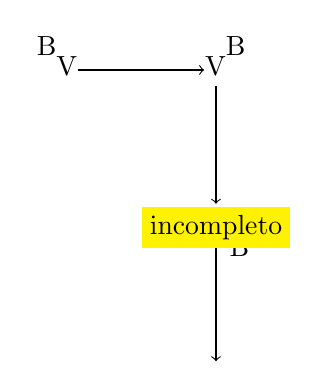
\begin{tikzpicture}
		\node[anchor=north west] at (0,0) {V};
		\node at (0,0) {B};
		\draw[->] (0.4,-0.3) -- (2,-0.3); % f sull linea
		\node[anchor=north east] at (2.4,0) {V};
		\node at (2.4,0) {B};
		\draw[->] (2.15,-0.5) -- (2.15,-2); % idv a destra della linea
		\node[anchor=north west] at (2.2,-2.3) {B'};
		\node at (2.15,-2.3) {V};
		\draw[->] (2.15,-2.5) -- (2.15,-4); % f sotto la linea
		\node at (2.15,-2.3) {\hl{incompleto}};

	\end{tikzpicture}

$det(\M_{B'}(f))=det(\M_{B'B}(idv)M_B(f)\M_{BB'}(idv))=det(\M_{B'B}(idv))det(\M_B(f))det(\M_{BB'}(f))=\frac{1}{\bar{det(\M_{BB'}(idv))}}\cdot det(\M_B(f))\cdot\bar{det(\M_{BB'}(idv))}$

	\ul{Partiamo da un esempio}

	Sia $f:\R^2\rightarrow\R^2$

$B=\{v_1=(1,1),v_2=(1,-1)\}$

$\M_B(f)=\begin{pmatrix}2&0\\0&-1\end{pmatrix}$, matrice diagonale

$f(v_1)=\begin{pmatrix}2&0\\0&-1\end{pmatrix}\begin{pmatrix}1\\0\end{pmatrix}=\begin{pmatrix}2\\0\end{pmatrix}=2v_1$

$f(v_1)=\begin{pmatrix}2&0\\0&-1\end{pmatrix}\begin{pmatrix}0\\1\end{pmatrix}=\begin{pmatrix}0\\-1\end{pmatrix}=-v_2$

$f(v_1+v_2)=\begin{pmatrix}2&0\\0&-1\end{pmatrix}\begin{pmatrix}1\\1\end{pmatrix}=\begin{pmatrix}2\\-1\end{pmatrix}=2v_1-v_2$

	\hl{disegno geometrico con vettori}

	Autovalore

	Autovettori

	Autospazio

	Operatore diagonale



	\Def{Sia $\V$ uno spazio vettoriale su $\K$}{
		Un endomorfismo $f\in End(\V)$ si dice \ul{diagonalizzabile} se esiste una base $B=\{v_1,\cdots,v_n\}$ di $\V$ tale che $\M_B(f)$ sia una matrice diagonale, cioè della forma

		$\begin{pmatrix}
				\lambda_1 & 0         & 0         \\
				0         & \lambda_2 & 0         \\
				0         & 0         & \lambda_n
			\end{pmatrix},\lambda_i\in\K$

		Se ciò avviene $B$ è detta una base diagonalizzante di $f$ e $\forall v_i\in B$ si ha

		$f(v_i)=\lambda_iv_i$

		$\lambda_i$ autovalore, $v_i$ autovettore
	}

	\Def{Sia $\V$ uno spazio vettoriale e sia $f\in End(\V)$.}{
		Un vettore $v\in\V$ si dice un \ul{autovettore} di $f$ se $v\not=0_\V$ e se $\exists\lambda\in\K$ tale che $f(v)=\lambda v$

		$\lambda$ è detto \ul{autovalore} di $f$ relativo all'autovettore $v$

		Il sottoinsieme di $\K$ costituito dagli autovalori di $f$ è detto \ul{spettro} di $f$.
	}

	\Esempio{
		\begin{itemize}
			\item $f=idv\in End(\V),dim(\V)=n$.\\
			      Per ogni base $B$ di $\V$\\
			      $\M_B=I_n\Rightarrow idv$ è diagonalizzabile.\\
			      $\forall v\in\V, id(v)=v=1\cdot v$\\
			      Quindi ogni $v\in\V\backslash\{0_\V\}$ è un autovettore di $idv$ di autovalore 1.
			\item \hl{incompleto}
		\end{itemize}
	}
	\section{13/05/22}
	\Def{Sia $\V$ uno spazio vettoriale su $\K$.}{
		Sia $f\in End(\V)$ un endomorfismo. Un vettore $v\in\V$ si dice autovettore se $v\not=0_\V$ e se $\exists\lambda\in\K$ tale che $f(v)=\lambda v$.

		Lo scalare $\lambda$ si dice autovalore di $f$ relativo all'autovettore $v$.

		Il sottoinsieme di $\K$ costituito dagli autovalori di $f$ è detto \ul{spettro} di $f$.

		L'endomorfismo $f$ si dice \ul{diagonalizzabile} se possiede una base $B=\{v_1,\cdots,v_n\}$ di autovettori, cioè se $\M_B(f)=\begin{pmatrix}
				\lambda_1 & 0         \\
				\hspace*{2em}\ddots   \\
				0         & \lambda_n
			\end{pmatrix}$

		Una tale base si dice base diagonale.
	}

	\paragraph*{Proposizione}: Siano $v_1,v_2\in\V$ due autovettori relativi allo stesso autovalore $\lambda$ per endomorfismo $f:\V\rightarrow\V$.

	Siano $\mu_1,\mu_2\in\K$ tali che $\mu_1v_1+\mu_2v_2\not=0_\V$.

	Allora $\mu_1v_1+\mu_2v_2$ è un autovettore di autovalore $\lambda$.

	\ul{dim}

	Mostriamo che $f(\mu_1v_1+\mu_2v_2)=\lambda(\mu_1v_1+\mu_2v_2)$.

$f(\mu_1v_1+\mu_2v_2)=\mu_1f(v_1)+\mu_2f(v_2)=\mu_1\lambda v_1+\mu_2\lambda v_2=\lambda(\mu_1v_1+\mu_2v_2)$ \boxed{}

	\Def{L'insieme}{
		$\V_\lambda:=\{v\in\V:v\text{ è un autovettore di }f\text{con autovalore}\lambda\}\cup\{0_\V\}$

		è un sottospazio vettoriale di $\V$ detto \ul{autospazio} relativo all'autovalore $\lambda$.
	}

	\paragraph*{Proposizione}: Se $v_1,\cdots,v_p\in\V$ sono autovettori relativi agli autovalori $\lambda_1,\cdots,\lambda_p\in\K$ e se questi $\lambda_i$ sono a due a due distinti, allora $v_1,\cdots,v_p$ sono linearmente indipendenti

	\ul{Dim}: sulle note della prof (per induzione)

	\ul{Obiettivo}: Dato $f\in End(\V)$, determinare se $f$ è diagonalizzabile e, in tal caso, determinare una base diagonalizzante, ossia una base di autovettori.

	\ul{Problema}: Come determiniamo lo spettro di $f$?

	Sia $f\in End(\V)$. Sia $\lambda$ un autovalore di $f$.

	Allora $\exists v\not=0_\V$ tale che

$f(v)=\lambda v\Leftrightarrow f(v)-\lambda v=0_\V\Leftrightarrow(f-\lambda idv)\rightarrow f-\lambda idv:\V\rightarrow\V\\\hspace*{25.4em}v\mapsto(f-\lambda idv)(v):=f(v)-\lambda v$ è un'applicazione lineare.

$\Leftrightarrow\text{teorema del rango}rg(f-\lambda idv)<n\\\Leftrightarrow det(f-\lambda idv)=0$7

	Sia $B$ una base di $\V$. Allora:

$det(f-\lambda idv)=0\Leftrightarrow det(\M_B(f-\lambda idv))=0\Leftrightarrow def(\M_B(d)-\lambda I_n)=0$

	\Def{Sia $A=(a_ij)\in\M_n(K)$ e sia $T$ un'indeterminata.}{
		Il determinante $P_A(T):=det(A-TI_n)=\begin{pmatrix}
				a_11   & a_12   & \cdots & a_1n   \\
				a_21   & a_22   & \cdots & a_2n   \\
				\vdots & \vdots & \ddots & \vdots \\
				a_n1   & a_n2   & \cdots & a_nn
			\end{pmatrix}$
		è un polinomio di grado $n$ in $T$ detto \ul{polinomio caratteristico} di $A$.

		Siano $f\in End(\V)$, $B$ una base di $\V$ e $A=M_B(f)$, allora $P_A(T)$ è il polinomio caratteristico di $f$ e si denota $P_f(T)$
	}

	\paragraph*{Osservazione}: Il polinomio caratteristico di un endomorfismo è indipendente dalla base scelta

	\paragraph*{Proposizione}: Sia $\V$ uno spazio vettoriale di dim $n$ e sia $f\in End(\V)$.

	Allora $\lambda$ è un autovalore di $f\Leftrightarrow\lambda$ è una radice di $P_f(T), (P_f(\lambda)=0)$.

	\paragraph*{Osservazione}: $P_f(T)\in\K[T]$ di grado $n$.

	Quindi $P_f(T)$ ha al più $n$ radici in $\K$.

	Ne segue che $f$ ha al più $n$ autovalori distinti.

	\paragraph*{Ricorda}:
	\begin{itemize}
		\item $\lambda$ è un autovalore di $f\in End(\V)\Leftrightarrow P_f(T)=0$.
		\item $\V_\lambda(f)=Ker(f-\lambda idv)$\begin{itemize}
			      \item $v=0_\V$
			      \item $v:f(v)=\lambda v\Leftrightarrow(f-\lambda idv)(v)=0_\V$
		      \end{itemize}
	\end{itemize}

	\Esempio{
		$f:\R^3\rightarrow\R^3$

		\hspace*{-2.3em}$(x,y,z)\mapsto(y-z,-x+2y,x-y+2z)$

		$B$: base canonica di $\R^3$:
		\begin{itemize}
			\item scrivere $M_B(f)$
			\item calcolare il polinomio caratteristico $P_f(T)$
			\item trovare le radici di $P_f(T)$ in $\R^3$
		\end{itemize}

		$M_B(f)=\begin{pmatrix}
				0  & 1  & -1 \\
				-1 & 2  & -1 \\
				1  & -1 & 2
			\end{pmatrix}$

		$P_f(T)=\begin{pmatrix}
				-T & 1   & -1  \\
				-1 & 2-T & -1  \\
				1  & -1  & 2-T
			\end{pmatrix}$\hl{incompleto}
	}
	\Def{Sia $\V$ uno spazio vettoriale su $\K,dim(\V)=n$}{
		Sia $f\in End(\V)$ e sia $\lambda\in\K$ un autovalore di $f$.

		Allora $dim(\V_\lambda(f))$ è detta \ul{molteplicità geometrica} di $\lambda$ per $f$.

		La \ul{molteplicità algebrica} di $\lambda$ per $f$ è la molteplicità di $\lambda$ come radice di $P_f(T)$.

		(molteplicità geometria $\le$ molteplicità algebrica)
	}
	\paragraph*{Teorema} $\V, dim(\V)=n,f\in End(\V),Spec(f)=\{\lambda_1,\cdots,\lambda_k\}$ (insieme degli autovalori)

	Allora:

$dim(V_{\lambda_1}(f))+\cdots+dim(V_{\lambda_k}(f))\le n$

	e l'uguagliansa sussiste se e solo se $f$ è diagonalizzabile.

	In tal caso:

$V=V_{\lambda_1}(f\oplus\cdots\oplus V_{\lambda_k}(f))$.

	Ne segue che una base diagonalizzante per $f$ è data dall'unione delle basi di ciascun autospazio.

	\paragraph*{Corollario}: Se $dim(V)=n$ e $f\in End(V)$ possiede $n$ autovalori, allora $f$ è diagonalizzabile.

\hl{esempio mancante}
\section{18/05/22}
\hl{incompleto}
\section*{Fine}
Ultimamente gli appunti sono pieni di grafici, mi è difficile prendere appunti, quindi lascio la scrittura di questo file al me del futuro che scriverà direttamente ricopiando gli appunti della professoressa.
Inoltre sarebbe necessaria una revisione approfondita di tutto il file









\end{document}
